\documentclass[conference]{IEEEtran}
\IEEEoverridecommandlockouts

\pagestyle{plain} % add line numbers

%%\setlength{\emergencystretch}{2pt}
%% \usepackage[font=small]{caption}
\usepackage{colortbl}
\usepackage{multirow}
\usepackage{subcaption}
\usepackage{listings}
\usepackage{comment}
\usepackage{adjustbox}
\usepackage{booktabs}
\let\labelindent\relax
\usepackage[inline]{enumitem}
\usepackage{ textcomp }
\usepackage{wrapfig}
%% \usepackage{listings}
%% %%%%%%%%%%%%% code listing
%% \renewcommand{\ttdefault}{pcr}
%% \lstset{
%%   basicstyle=\scriptsize\ttfamily,
%%   keywordstyle=\scriptsize\ttfamily\bfseries,
%%   language=Java,             % choose the language of the code
%%   frame=single,              % adds a frame around the code
%%   aboveskip=0pt,
%%   belowskip=0pt,
%%   breaklines=true,           % sets automatic line breaking
%%   breakatwhitespace=false,   % sets if automatic breaks should only happen at
%%   showspaces=false,
%%   %numbersep=5pt,              % Abstand der Nummern zum Text
%%   %tabsize=2,                  % Groesse von Tabs
%%   %extendedchars=true,         %
%%   %breaklines=true,            % Zeilen werden Umgebrochen
%%   keywords=[2]{class, incorporateUserFeedback, testPushPop, testPopPush},
%% }
%% \usepackage{fancyvrb}\fvset{fontsize=\small}
%% \usepackage{tikz}
%% \usetikzlibrary{chains,shadows.blur}
%% \usetikzlibrary{patterns}
%% \usepackage[ruled, vlined, linesnumbered]{algorithm2e}
%% \usepackage{algorithmic}
%% \usepackage{array}
%% \usepackage{mathtools}
%% \usepackage{url}
%% \usepackage{xstring}
\usepackage{hyperref} 
%% \usepackage[T1]{fontenc}
%% \usepackage{seqsplit}
%% Colors
\usepackage{color}
%% \definecolor{bgBlock}{rgb}{0.22,0.15,0.49}
%% \definecolor{bgBlockAlert}{rgb}{0.99,0.84,0.31}
%% \definecolor{fgBlockAlert}{rgb}{0.22,0.15,0.49}
%% \definecolor{fgBlock}{rgb}{0.99,0.84,0.31}
%% \definecolor{darkred}{rgb}{0.5,0,0}
%% \definecolor{darkgreen}{rgb}{0,0.5,0}
%% \definecolor{darkblue}{rgb}{0,0,0.5}
\definecolor{LightGray}{rgb}{0.75,0.75,0.75}
\definecolor{VeryLightGray}{rgb}{0.90,0.90,0.90}
\definecolor{ForestGreen}{rgb}{0.13,0.54,0.13}

%% \usepackage{float}
%% \usepackage{caption}
%% \usepackage{subcaption}
\usepackage{cite}
%% \usepackage{amsmath,amssymb,amsfonts}
%% \usepackage{amsthm}
\usepackage[noend]{algpseudocode}
\usepackage{algorithm}
%% \usepackage{graphicx}
%% \usepackage{textcomp}
%% \usepackage{xcolor}
%% \usepackage{cancel}
\usepackage{tikz}
\usetikzlibrary{matrix,chains,positioning,decorations.pathreplacing,arrows}
\usepackage[skins]{tcolorbox}
%% DON'T DO THIS IN ACM STYLE
%%\renewcommand{\baselinestretch}{0.964}

\newcommand{\tname}{\textsc{Shaker}} %% technique name
\newcommand{\rerun}{ReRun}
\newcommand{\rerunN}{ReRun$_N$}
\newcommand{\ngen}{$\mathit{NG}$}
\newcommand{\sng}{stress-ng}
\newcommand{\artifactUrl}{\url{https://github.com/shaker-project/shaker}}
\newcommand{\greedy}{Greedy}

\newcommand{\tr}{$\mathit{TR}$}

\newcommand{\Mar}[1]{[\textbf{Marcelo}:{\color{magenta} #1}]}
\newcommand{\Leo}[1]{[\textbf{Leopoldo}:~{\color{blue} #1}]}
\newcommand{\Den}[1]{[\textbf{Denini}:~{\color{brown} #1}]}

\newcommand{\CodeIn}[1]{\begin{footnotesize}\texttt{#1}\end{footnotesize}}
\newcommand{\Fix}[1]{\textbf{[\color{red}#1]}}
\newcommand{\Ignore}[1]{}
\newcommand{\myeg}{e.g.}
\newcommand{\ie}{i.e.}
\newcommand{\etc}{etc.}

\newcommand{\ann}{ANN}
\newcommand{\bmc}{BMC}
\newcommand{\ibmc}{IBMC}
\newcommand{\etal}{et al.}
\renewcommand{\algorithmicrequire}{\textbf{Input:}}
\renewcommand{\algorithmicensure}{\textbf{Output:}}
\newtheorem{theorem}{Theorem}[section]
\newtheorem{corollary}{Corollary}[theorem]
\newtheorem{lemma}[theorem]{Lemma}

%\lstset{language=C,basicstyle=\small}
\lstset{language=C,basicstyle=\small\ttfamily}
\lstset{numbers=left, numberstyle=\tiny, stepnumber=1, numbersep=5pt}
\lstset{tabsize=2}
\lstset{firstnumber=1}
\lstset{frame=single}
%\lstset{float}
\lstset{
  basicstyle=\scriptsize\ttfamily,
  keywordstyle=\scriptsize\ttfamily\bfseries,
  language=C,             % choose the language of the code
  %frame=, %single             % adds a frame around the code
  aboveskip=0pt,
  belowskip=0pt,
  breaklines=true,           % sets automatic line breaking
  breakatwhitespace=false,   % sets if automatic breaks should only happen at
  showspaces=false,
  %tabsize=2,                  % Groesse von Tabs
  %extendedchars=true,         %
  %breaklines=true,            % Zeilen werden Umgebrochen
  %keywords=[2]{},
  keywords={},
  %% numbersep=0pt,              % Abstand der Nummern zum Text  
  %% numbers=left,
  escapeinside={\%*}{*)},          % if you want to add LaTeX within  % your code
  morekeywords={public, for, typedef, void, float, unsigned, short, int, ushort, assert,uchar,begin_thread,end_thread,join_thread,atomic,assume,static,extern,int,_Bool,return}  
}

\newcommand{\Space}[1]{}

% other paragraphs
\newcommand{\Contrib}[1]{$\star$#1}


%% numbers 
\newcommand{\numprojects}{11}
\newcommand{\totalTests}{1,298}
\newcommand{\numprojectsWithFlakies}{7}
\newcommand{\numNewFlakies}{30}
\newcommand{\numReRuns}{50}
\newcommand{\numflakytestsds}{75}
\newcommand{\percFlakyTestSds}{5.78}
\newcommand{\numflakytraining}{35}
\newcommand{\numflakytesting}{40}
\newcommand{\numReRunstraining}{3}
\newcommand{\numReRunstrainingLONG}{3}
\newcommand{\numTestsAntenna}{250}
\newcommand{\numTrainingSet}{35}
\newcommand{\numTestingSet}{40}
\newcommand{\numRandomConfigs}{50}
\newcommand{\threshold}{0.66}
\newcommand{\numExecutionsRQThree}{10}
\newcommand{\numTotalNewFlaky}{61}
%RQ4
\newcommand{\numFlakyDetectedShaker}{38}
\newcommand{\numFlakyDetectedReRun}{15}
\newcommand{\percFlakyDetectedShaker}{95\%}
\newcommand{\percFlakyDetectedReRun}{37.5\%}


%%numbersRQ3
\newcommand{\configsMHS}{$\{c_1, c_18, c_20, c_17\}$}
\newcommand{\configsGreed}{$\{c_18, c_20, c_22, c_32\}$}
\newcommand{\configsRandom}{$\{c_1,...\}$}


\def\BibTeX{{\rm B\kern-.05em{\sc i\kern-.025em b}\kern-.08em
    T\kern-.1667em\lower.7ex\hbox{E}\kern-.125emX}}
    
\begin{document}

\title{Shake It! Detecting Flaky Tests Caused by Concurrency with Shaker}
%\title{Optimized \rerun{} to Find \\ Time-Constrained Flaky Tests}

\author{\IEEEauthorblockN{Denini Silva, Leopoldo Teixeira, Marcelo d'Amorim}
% Pessoal, eu removi parte dos dados institucionais pelas razoes abaixo:
%  (1) muita informacao faz com o que o pessoal esqueca da marca
%  (2) entendo que o credito para UFPE seja suficiente. 
%  (3) o pessoal consegue encontrar info na web
\IEEEauthorblockA{Federal University of Pernambuco, Brazil\\
\{dgs,lmt,damorim\}@cin.ufpe.br}
} % Informatics Center, (CIn-UFPE), Recife-PE 

\makeatletter
\newcommand{\linebreakand}{%
  \end{@IEEEauthorhalign}
  \hfill\mbox{}\par
  \mbox{}\hfill\begin{@IEEEauthorhalign}
}
\makeatother
\maketitle


%%%%%%%%%%%%%%%%%%%%%%%
%% Anonymous authors!
%%%%%%%%%%%%%%%%%%%%%%%
%\author{\IEEEauthorblockN{Marcio Augusto Guimar{\~a}es$^{\star}$\quad{}Leo Fernandes$^{\ddagger}$\quad{}M{\'a}rcio Ribeiro$^{\star}$\quad{}Marcelo d'Amorim$^{\dagger}$\quad{}Rohit Gheyi$^{\ast}$}
%\IEEEauthorblockA{
%$^{\star}$Federal University of Alagoas, Macei{\'o}-AL, Brazil\\
%$^{\ddagger}$Federal Institute of Alagoas, Macei{\'o}-AL, Brazil\\
%$^{\dagger}$Federal University of Pernambuco, Recife-PE, Brazil\\
%$^{\ast}$Federal University of Campina Grande, Campina Grande-PB, Brazil \\
%\{masg, marcio\}@ic.ufal.br\quad{}leonardo.oliveira@ifal.edu.br\quad{}damorim@cin.ufpe.br\quad{}rohit@dsc.ufcg.edu.br}}

\begin{abstract}
% context
A test is said to be flaky when it non-deterministically passes or fails. Test flakiness negatively affects the effectiveness of regression testing and, consequently, impacts software evolution. 
% problem
Detecting test flakiness is an important and challenging problem. \rerun{} is the most popular approach in industry to detect test flakiness. It re-executes a test suite on a fixed code version multiple times, looking for inconsistent outputs across executions. Unfortunately, \rerun{} is costly and unreliable.
%needs several executions to capture low probability flaky tests.
% solution
This paper proposes \tname{}, a lightweight technique to improve the ability of \rerun{} to detect flaky tests. \tname{} adds noise in the execution environment (e.g., it adds stressor tasks to compete for the CPU or memory). It builds on the observations that concurrency is an important source of flakiness and that adding noise in the environment can interfere in the ordering of events and, consequently, influence on the test outputs.
% evaluation
We conducted experiments on a data set with \numprojects\ Android apps. Results are very encouraging. \tname\ discovered many more flaky tests than \rerun{} (\percFlakyDetectedShaker{} and \percFlakyDetectedReRun{} of the total, respectively) and discovered these flaky tests much faster. In addition, \tname\ was able to reveal \numTotalNewFlaky\ new flaky tests that went undetected in \numRandomConfigs\ re-executions with \rerun. 
%We conducted experiments on a data set with \numflakytestsds{} flaky tests of \numprojects{} open source Android apps. Results are encouraging. We found that \tname{} detected $\sim$85\% of all flaky tests from our data set in $\sim$10\% of the time \rerun{} needed for that task. Furthermore, we ran \tname{} on this same set of apps and found \numNewFlakies{} new flaky tests that \numReRuns{} re-executions of the test suite missed. 
\end{abstract}

\begin{IEEEkeywords}
test flakiness, regression testing, noise
\end{IEEEkeywords}%\documentclass[10pt, conference, letter]{IEEEtran}

%%%ABSTRACT FOR CAMERA-READY SUBMISSION
% A test is said to be flaky when it non-deterministically passes or fails. Test flakiness negatively affects the effectiveness of regression testing and, consequently, impacts software evolution. Detecting test flakiness is an important and challenging problem. ReRun is the most popular approach in industry to detect test flakiness. It re-executes a test suite on a fixed code version multiple times, looking for inconsistent outputs across executions. Unfortunately, ReRun is costly and unreliable. This paper proposes Shaker, a lightweight technique to improve the ability of ReRun to detect flaky tests. Shaker adds noise in the execution environment (e.g., it adds stressor tasks to compete for the CPU or memory). It builds on the observations that concurrency is an important source of flakiness and that adding noise in the environment can interfere in the ordering of events and, consequently, influence on the test outputs. We conducted experiments on a data set with 11 Android apps. Results are very encouraging. Shaker discovered many more flaky tests than ReRun (95\% and 37.5\% of the total, respectively) and discovered these flaky tests much faster. In addition, Shaker was able to reveal 61 new flaky tests that went undetected in 50 re-executions with ReRun.


%%%%%%%%%%%%%%%%%%%%%%%%%%%%%%%%%%%%%%%%%%%%%%%%%%
%% Intro
%%%%%%%%%%%%%%%%%%%%%%%%%%%%%%%%%%%%%%%%%%%%%%%%%%

\section{Introduction}
\label{sec:intro}

A test is said to be \emph{flaky} when it non-deterministically passes or fails depending on the running environment~\cite{john-mico-google2016}. For example, a test may fail or pass depending on the availability of a server that the test itself has spawned---the test passes if the server is up-and-running at the point the test makes a request to the server and it fails, otherwise. 

Test flakiness hurts software testing practice in multiple ways. For example, Thorve~\etal{}~\cite{thorve2018empirical} found that, because of test flakiness, developers lost trust in test results, choosing to ignore test failures altogether sometimes. Even ignoring failures of known flaky tests or ignoring previously classified flaky tests (\ie{}, not executing those tests) can be dangerous as those tests could reveal bugs in code. Furthermore, ignoring flakiness can produce the effect of observing even more failures to be analyzed during software evolution. For example, Rahman and Rigby~\cite{rahman-rigby-fse2018} found that when developers ignored flaky test failures during a build, the deployed build experienced more crashes than builds that did not contain any flaky test failures. 
Test flakiness is a huge problem in industry. Most test failures at Google are due to flaky tests~\cite{john-mico-google2016,jeff-listfield-google2017}. At Microsoft, the presence of flaky tests also imposes a significant burden on developers. Wing~\etal{}~\cite{wing-etal-issta11} reported that 58 Microsoft developers involved in a survey considered flaky tests to be the second most important reason, out of 10 reasons, for slowing down software deployments. Finally, Facebook considers flakiness detection a priority~\cite{DBLP:conf/scam/HarmanO18}. 

\rerun\ is the most popular approach in industry to detect test flakiness~\cite{john-mico-google2016,flakiness-at-spotify}. 
It reruns tests multiple times. A test that failed and then passed is considered flaky, and vice-versa. The status of a test that persistently failed is unknown, but developers typically treat this scenario as a problem in application code as opposed to a bug in test code. Unfortunately, \rerun{} is unreliable and expensive. It is unreliable because it is hard to determine the number of reruns to find discrepancy in outputs. It is expensive because rerunning tests consumes a lot of computing power. Google, for example, uses 2-16\% of its testing budget just to rerun flaky test~\cite{john-mico-google2016}. Researchers have proposed various techniques to identify flaky tests. Bell~\etal{}~\cite{bell2018d} proposed DeFlaker, a technique that determines that a test is flaky if the output of a test has changed even though there was no change in the code reachable from the execution trace. Note that DeFlaker cannot capture flakiness in test cases not impacted by changes and that change-impacted flaky tests do not reveal flakiness necessarily. Pinto~\etal~\cite{pinto-etal-msr2020} proposed the use of text processing and classification to statically identify likely flaky test cases from the keywords they use. 
%Important to note that the technique provides indication of likely flakiness, not a verdict. 
%Overall, existing approaches suffer from different limitations. 

This paper proposes \tname, a lightweight technique to improve the ability of \rerun\ to detect flaky tests.
\tname\ adds noise in the execution environment with the goal of provoking failures in time-constrained tests.  For example, it adds stressor tasks to compete with the test execution for the CPU or memory. \tname{} builds on the observations that concurrency is an important source of flakiness~\cite{Luo:2014:EAF:2635868.2635920,dong2020concurrencyrelated} and that adding noise in the environment can interfere in the ordering of events related to test execution and, consequently, influence on the test outputs. The process of detecting flaky tests consists of two steps. In the first \emph{offline} step, \tname{} uses a sample of tests known to be flaky to search for configurations of a noise generator to be used for revealing flakiness in new tests. To that end, \tname\ first builds a probability matrix encoding the relation between flaky tests and noise configurations. The matrix shows the probability of a test failing when executed with a given noise configuration. Then, \tname{} uses that matrix to search for sets of configurations that reveals the highest number of flaky tests. In the second \emph{online} step, \tname{} uses those configurations to find time-constrained flaky tests in the project of interest.

\begin{figure*}[t!]
\begin{lstlisting}[language=Java, caption=AntennaPod Test,label=AntennaPodTest, escapechar=|, keywords={@Test, perform, await}]
@Test
public void testReplayEpisodeContinuousPlaybackOff() throws Exception {
 setContinuousPlaybackPreference(false);|\label{line:continuousplayback}|
 uiTestUtils.addLocalFeedData(true);|\label{line:adddata}|
 activityTestRule.launchActivity(new Intent());
 //Navigate to the first episode in the list of episodes and click
 openNavDrawer();|\label{line:nav-start}|
 onDrawerItem(withText(R.string.episodes_label)).perform(click());
 onView(isRoot()).perform(waitForView(withText(R.string.all_episodes_short_label), 1000));
 onView(withText(R.string.all_episodes_short_label)).perform(click());
 final List<FeedItem> episodes = DBReader.getRecentlyPublishedEpisodes(0, 10);
 Matcher<View> allEpisodesMatcher = allOf(withId(android.R.id.list), isDisplayed(), hasMinimumChildCount(2));
 onView(isRoot()).perform(waitForView(allEpisodesMatcher, 1000));
 onView(allEpisodesMatcher).perform(actionOnItemAtPosition(0, clickChildViewWithId(R.id.secondaryActionButton)));|\label{line:nav-finish}|
 FeedMedia media = episodes.get(0).getMedia();
 Awaitility.await().atMost(1, TimeUnit.SECONDS).until( () -> media.getId() == PlaybackPreferences.getCurrentlyPlayingFeedMediaId());|\label{line:awitibility}| ... }
\end{lstlisting}
\end{figure*}


We conducted experiments on a data set with \numflakytestsds{} flaky tests of \numprojects{} open source Android apps. Preliminary results provide early evidence that \tname\ is promising. \tname\ discovered many more flaky tests than \rerun{} (\percFlakyDetectedShaker{} and \percFlakyDetectedReRun{} of the total from our data set, respectively) and discovered these flaky tests much faster than \rerun. \tname{} discovered 85\% of the total number of possible flakies in 10\% of the average time \rerun\ took to find its maximum number of flakies. In addition, \tname\ was able to reveal \numTotalNewFlaky\ new flaky tests that went undetected in \numRandomConfigs\ re-executions with \rerun. This paper makes the following contributions:

\begin{itemize}[topsep=.2ex,itemsep=.2ex,leftmargin=0.8em]

\item[\Contrib{}]\textbf{Approach.} We proposed a simple lightweight approach to find time-constrained flaky tests by introducing noise in the test environment where tests will be executed.
  
\item[\Contrib{}]\textbf{Implementation.}~We developed a tool implementing \tname{} (available per request due to double blindness).

%\Mar{Denini, if we have time it would be good to write some gradle/maven plugin. If not, we only make the optimization scripts available.}
  
\item[\Contrib{}]\textbf{Evaluation.} We evaluated \tname{} on \numprojects\ Android apps with encouraging results.

\item[\Contrib{}]\textbf{Artifacts.} Our scripts, data sets, and list of issues submitted to GitHub projects, are publicly available at the following link \textbf{\artifactUrl{}}.

\end{itemize}


%%%%%%%%%%%%%%%%%%%%%%%%%%%%%%%%%%%%%%%%%%%%%%%%%%
%% Examples
%%%%%%%%%%%%%%%%%%%%%%%%%%%%%%%%%%%%%%%%%%%%%%%%%%

\section{Examples}
\label{sec:example}

% \Mar{need to describe few compelling examples. @Denini, can you find two or three tests that we frequently detect flakiness (prob. higher than >.5) and it is difficult for rerun to find (prob. lower than .1)? @Leopoldo, can you dig into these examples and explain 1) why they are flaky (time constraints)?} \Leo{Working on Denini's examples.}

This section presents two examples of flaky tests in Android applications (apps) to motivate and illustrate \tname{}. Before introducing the examples, it is important to briefly explain concepts related to the Android OS. The execution of an Android app creates a separate process including an execution thread, typically called the \emph{main} thread, or the UI thread. This thread is responsible for handling events such as callbacks from UI interactions, callbacks associated with the lifecycle of components, \etc\ Any costly operation, such as network operations, should be offloaded to separate threads to avoid blocking the main thread, and consequently freezing the UI. Blocking the main thread for more than 5 seconds results in an Application Not Responding (ANR) error, which crashes the app. Consequently, \emph{asynchronous operations are common in Android apps}. Separate worker threads, responsible for these operations, are not allowed to manipulate the UI directly, which is responsibility of the main (UI) thread. Consequently, there must be coordination among worker threads and the main thread. Testing frameworks, such as Espresso~\cite{espresso-2020}, provide means to handle asynchronous operations. However, developers may fail to properly coordinate tasks from tests.

%

\subsection{AntennaPod}

%\begin{figure}[t!]
%    \centering
%    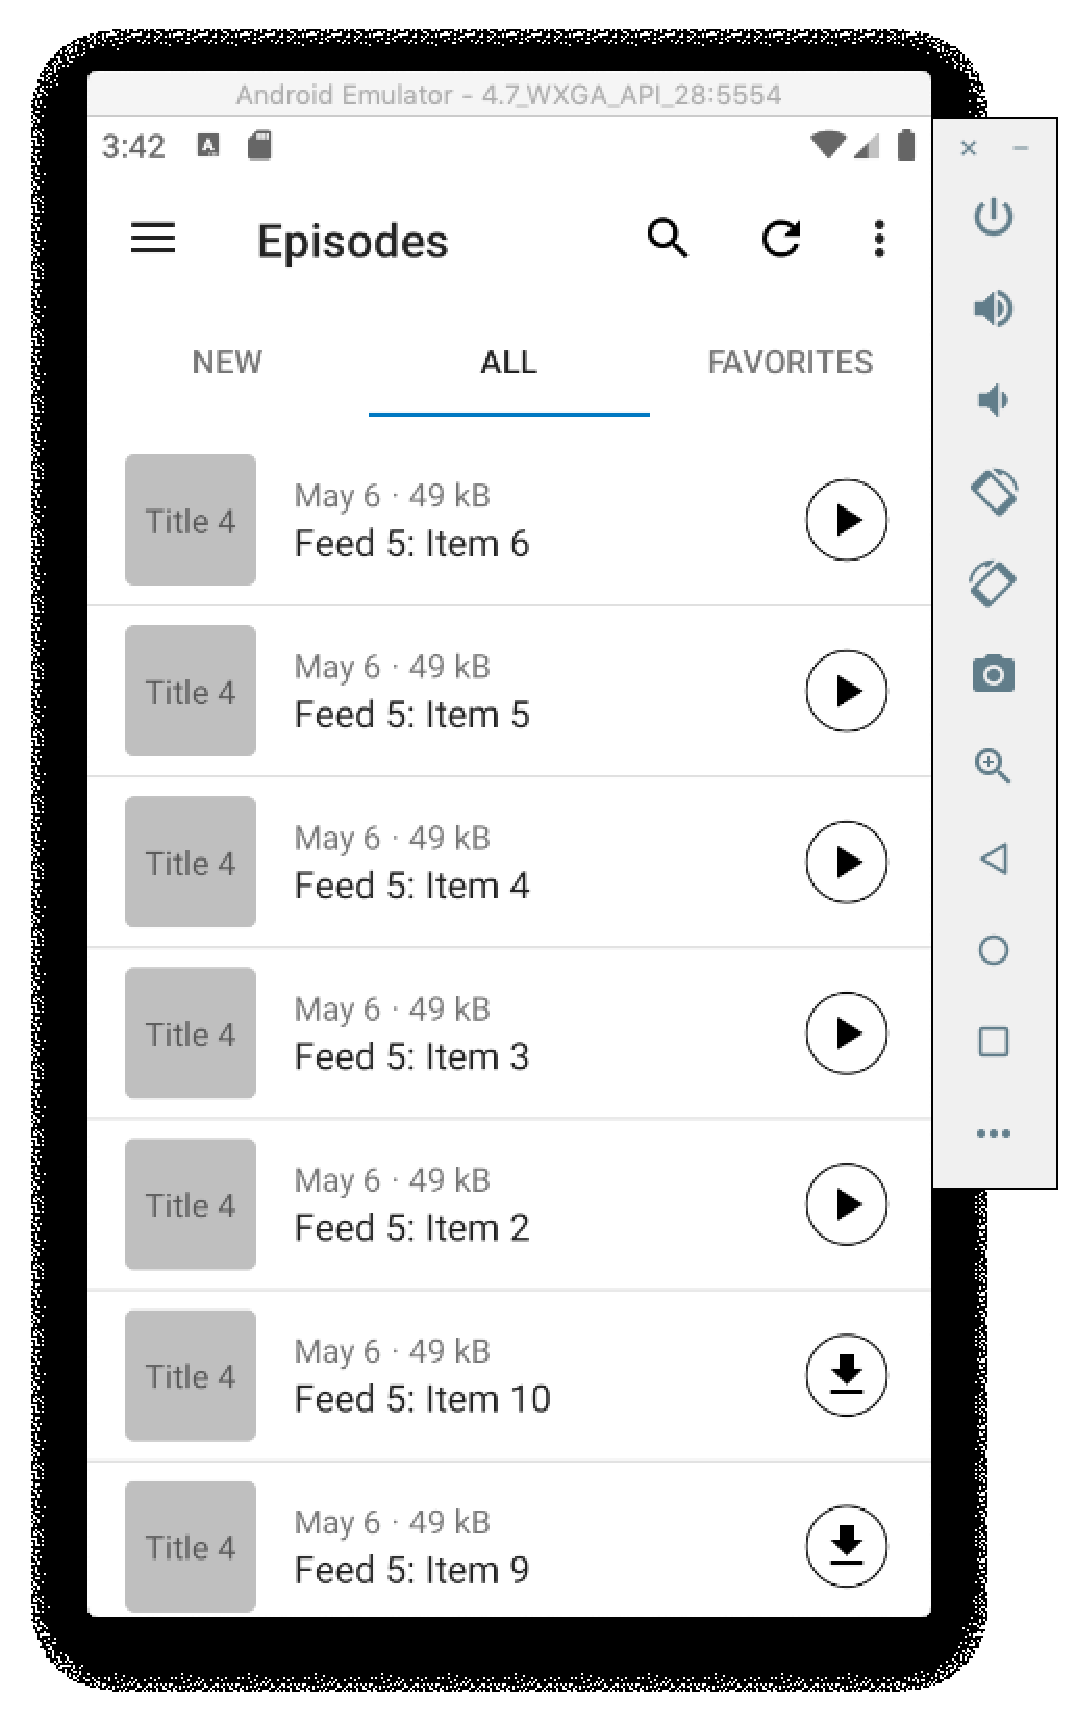
\includegraphics[width=5cm]{figs/antennapod.eps}
%    \caption{AntennaPod.}
%    \label{fig:antennapod}
%\end{figure}

\begin{figure*}[t!]
\begin{lstlisting}[language=Java, caption=Paintroid Test, label=PaintroidTest, escapechar=|, keywords={@Test, perform, performSelectTool, performOpenMoreOptions, performOpenToolOptionsView, performCloseToolOptionsView, await}]
@Test
public void testFullscreenPortraitOrientationChangeWithShape() {
 onToolBarView().performSelectTool(ToolType.SHAPE);|\label{line:selectShape}|
 setOrientation(SCREEN_ORIENTATION_PORTRAIT);|\label{line:setPortrait}|
 onTopBarView().performOpenMoreOptions();|\label{line:optionsMenu}|
 onView(withText(R.string.menu_hide_menu)).perform(click());|\label{line:fullScreen}|
 setOrientation(SCREEN_ORIENTATION_LANDSCAPE);|\label{line:setLandscape}| pressBack();|\label{line:pressBack}|
 onToolBarView().performOpenToolOptionsView().performCloseToolOptionsView();|\label{line:closeToolOptions}| }
\end{lstlisting}
\end{figure*}



\sloppy
AntennaPod~\cite{antennapod} is an open source podcast manager for Android supporting episode download and streaming. 
The AntennaPod app is implemented in Java in $\sim$50KLOC.
As of the date of submission,\footnote{Revision SHA dd5234c as per the time of submission.} the app had \numTestsAntenna{} GUI tests written in Espresso~\cite{espresso-2020} and UIAutomator~\cite{uiautomator-2020}. 

Listing~\ref{AntennaPodTest} shows a simplified version of a test that %\CodeIn{testReplayEpisodeContinuousPlaybackOff}, 
checks whether a podcast episode can be played twice. 
It uses the Awaitility library~\cite{awaitibility} to handle asynchronous events, such as I/O events related to notifications of media playback. Executing the statement at line~\ref{line:continuousplayback} turns off the continuous playback option. This stops the app from automatically playing the next episode in queue after it finishes the current one. The statement at line~\ref{line:adddata} then adds local data (e.g.{}, podcast feeds, images, and episodes) to the app whereas the execution of the statements at lines~\ref{line:nav-start}--\ref{line:nav-finish} navigate through the GUI objects with the effect of playing the first episode in the queue. Line~\ref{line:awitibility} shows an assertion based on the Awaitibility library. The assertion checks if the episode is being played and indicates that test execution should wait for at most one second to verify this (line~\ref{line:awitibility}). 
%This test is flaky, it fails depending on the state of the environment. It checks whether or not the episode is being played. 
When the play button is pressed (line~\ref{line:nav-finish}), the app runs a custom service in the background\footnote{Look for ``Thread'' in the \CodeIn{PlaybackService.java} file~\cite{antennapod-playback}.}---to load the media file from the file system and, subsequently, play the media to the user. These are typically expensive I/O operations. If the machine running the test is heavy-loaded, the 1 second limit may not be reached. Consequently, the execution of the test will fail with a  \CodeIn{ConditionTimeoutException} exception raised by the Awaitibility library. 

We ran this test case 50 times and found failures in 11 runs, \ie{}, 22\% of the cases. Considering this example, one would need to execute the test for more than four times to detect the failure with high probability. When configured to execute the test suite using only the most effective noisy \tname{} configuration, we were able to detect failure in the first execution of the test suite. Furthermore, we re-executed the test case for 50 times with this configuration and were able to detect flakiness in all of them. Although each individual execution of the test suite is more expensive with \tname, it requires fewer re-executions of the test suite to detect flakiness. For comparison, one non-noisy execution of this test case takes 11.08s whereas one execution of the test case under \tname{}'s noisy environment takes 20.2s, \ie{}, the execution without noise is $\sim$2x faster in this particular case. However, comparing the total execution time, we observed that \tname{} enabled the discovery of flakiness 2.49x (=50.3/20.2) faster and, more importantly, it required a single execution for that.

\subsection{Paintroid}

\sloppy
Paintdroid is a graphical paint editor application for Android implemented in Java in $\sim$25KLOC. As of its latest version,\footnote{Revision SHA 1f302a2 as per the time of submission} it had 250 Espresso tests. One of such tests 
%, \CodeIn{testFullscreenPortraitOrientationChangeWithShape}, 
checks whether some buttons can be clicked after changing the screen orientation. Listing~\ref{PaintroidTest} shows the test. It first selects the Shape drawing option~(line~\ref{line:selectShape}), and then sets the screen orientation to portrait~(line~\ref{line:setPortrait}). Then, it opens a menu that shows a list of options~(line~\ref{line:optionsMenu}) (e.g., option to save an image, option to export image to a file, etc). The test clicks on the full screen option~(line~\ref{line:fullScreen}), then it changes orientation to landscape~(line~\ref{line:setLandscape}), exits full screen mode~(line~\ref{line:pressBack}), and clicks on the tool options to again open a menu, and then close it~(line~\ref{line:closeToolOptions}). Note that there are no assertions in the test. The intention is to validate that the options remain clickable as the orientation changes from portrait to landscape.

% Some device configurations can change during runtime (such as screen orientation, keyboard availability, and when the user enables multi-window mode). When such a change occurs, Android restarts the running Activity ( onDestroy() is called, followed by onCreate()). The restart behavior is designed to help your application adapt to new configurations by automatically reloading your application with alternative resources that match the new device configuration. 
Like the previous example, this test can produce different results depending on the efficiency of the machine. More precisely, the click on the menu item~(line~\ref{line:fullScreen}) can be performed before or after the menu is rendered on the screen~(line~\ref{line:optionsMenu}). 
As expected, the test fails, throwing the \CodeIn{PerformException}, if the click is performed before the menu is shown. 
Changing screen orientation corresponds to a configuration change in Android.\footnote{\url{https://developer.android.com/guide/topics/resources/runtime-changes}} When a configuration change happens, Android destroys and recreates the current screen (represented by an \CodeIn{Activity} object). This happens because changing orientation might result in a different screen layout.%, therefore, it might need to load different resources. 
% This happens because Android method calls (\Fix{name which one}) are mostly asynchronous \Mar{why "mostly"? can we cite this?}. Moreover, animations might also impact Espresso tests due to introduced delays.\Mar{don't understand. are there animations here?}

We ran this test case for 50 times with \rerun\ and found failures in 4 runs (8\% of the cases). This example shows that, albeit practical and widely adopted in industry~\cite{Luo:2014:EAF:2635868.2635920,DBLP:conf/scam/HarmanO18,john-mico-google2016}, \rerun{} can be (1)~ineffective or (2)~costly to proactively detect flaky tests. Given that it takes 12.5 (=50/4) executions on average to find flakiness and each regular execution takes 5.54s, the aggregate cost to detect this flaky test with \rerun{} is 69.25s (=12.5*5.54). We also ran the test case for 50 times with \tname{} and found failures in 18 runs (26\% of the cases). As the test fails in every 2.78 (=50/18) executions and each execution with \tname\ takes 7.08s, the aggregate cost of \tname{} to find this flaky test is 19.68s (=2.78x7.08). Overall, \tname{} reveals the flaky test 3.52x faster than \rerun\ (=69.25/19.68) despite having the execution of the test case itself 1.28x (=7.08/5.54) slower.


%With \tname{}, we were able to find failures in 18 cases, \ie{} 36\%. In this test case, \tname{} increases the chances of finding fault by 4.5 times (8\% versos 36\%).

\section{\tname{}}
\label{sec:approach}


\sloppy
The goal of \tname{} is to detect flaky tests. The observation that motivates \tname{} is that many tests are flaky because of timing constraints in test executions~\cite{Luo:2014:EAF:2635868.2635920,thorve2018empirical,dong2020concurrencyrelated}, such as those from the examples. Our hypotheses are that 1)~such tests can be detected by adding noise in the environment where test cases will run and 2)~rerunning tests in a noisy environment will more promptly reveal flaky tests compared with rerunning tests without noise.

\begin{figure}[h]
    \centering
    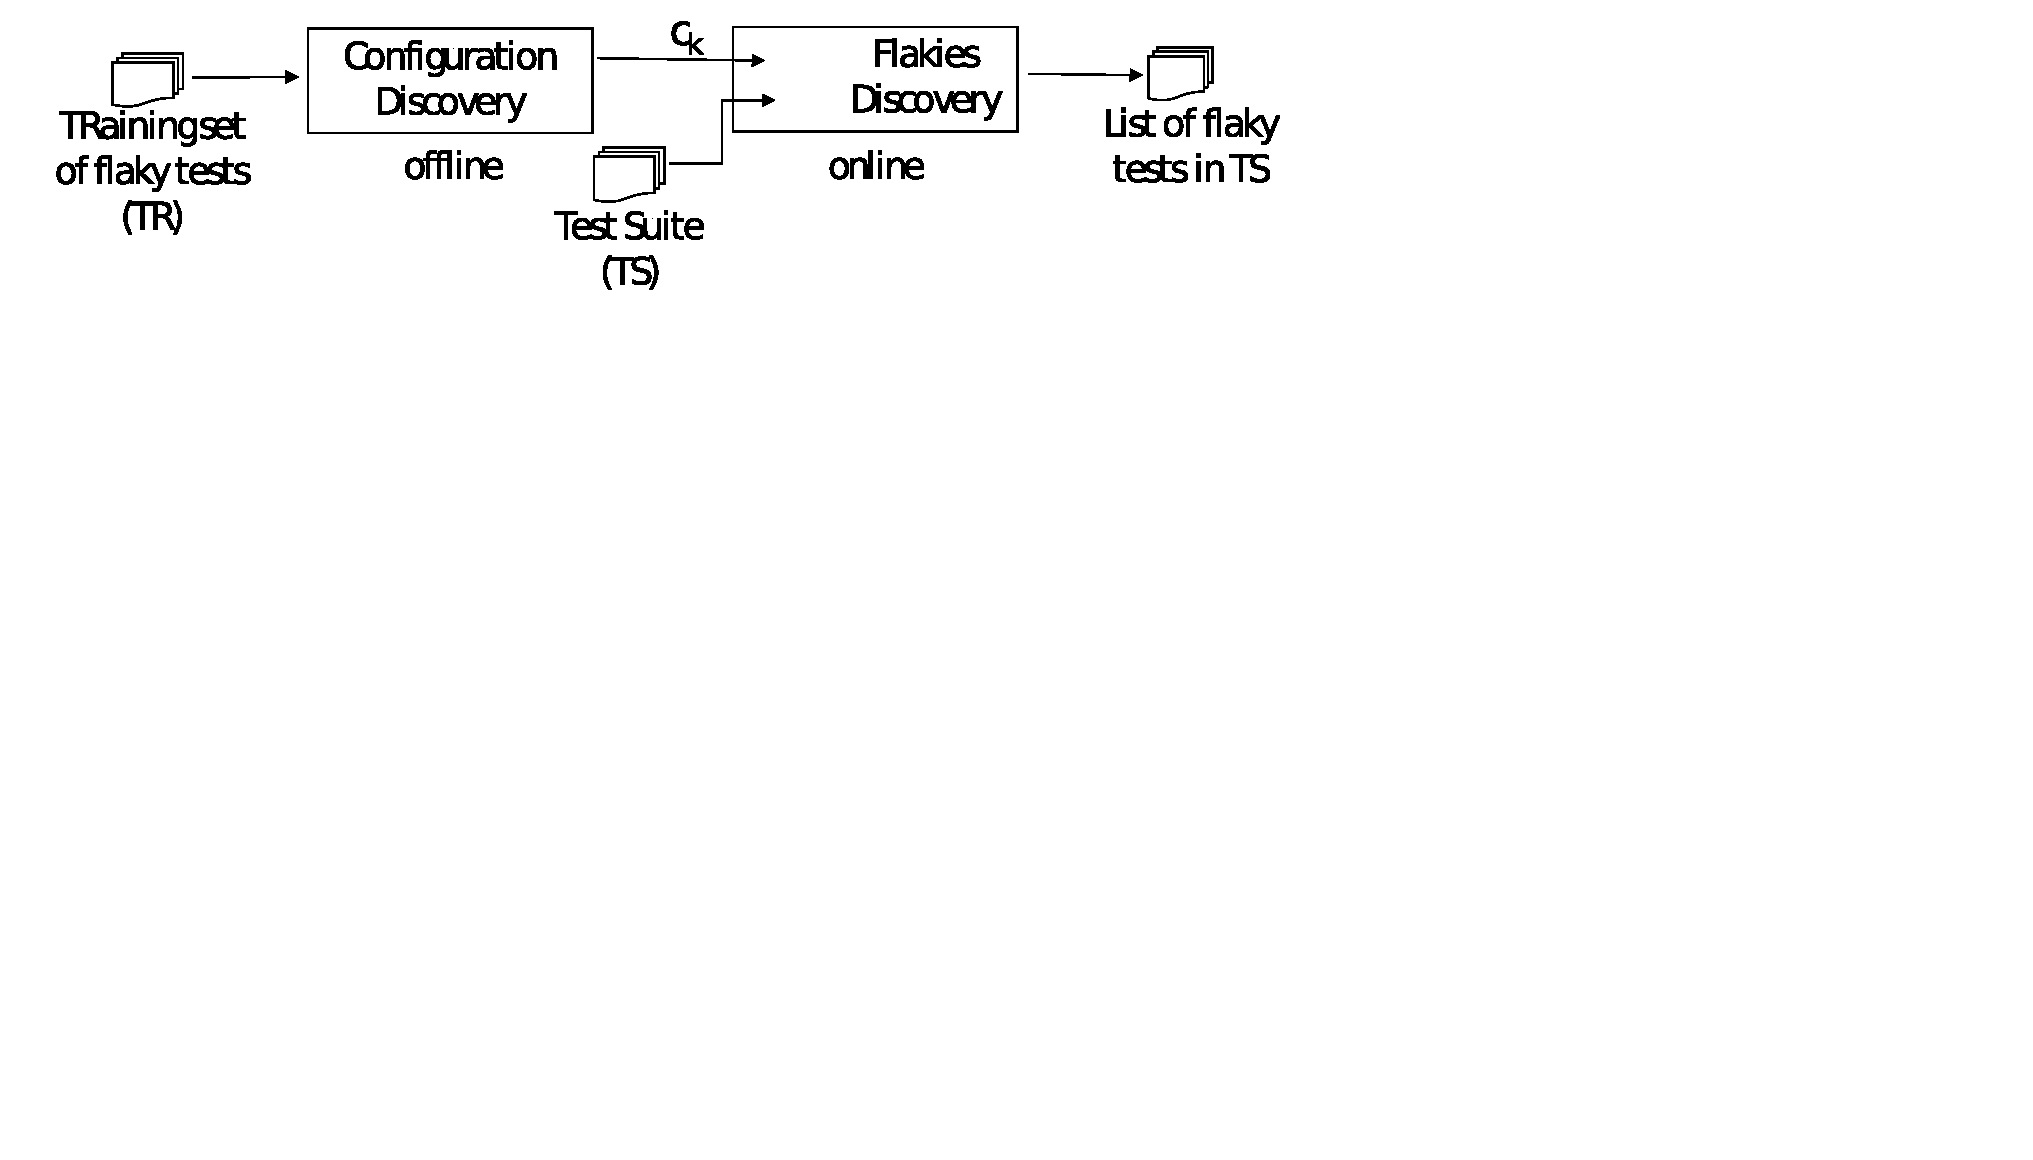
\includegraphics[trim=0 400 0 0,clip,width=0.75\textwidth]{figs/shaker.eps}
    % 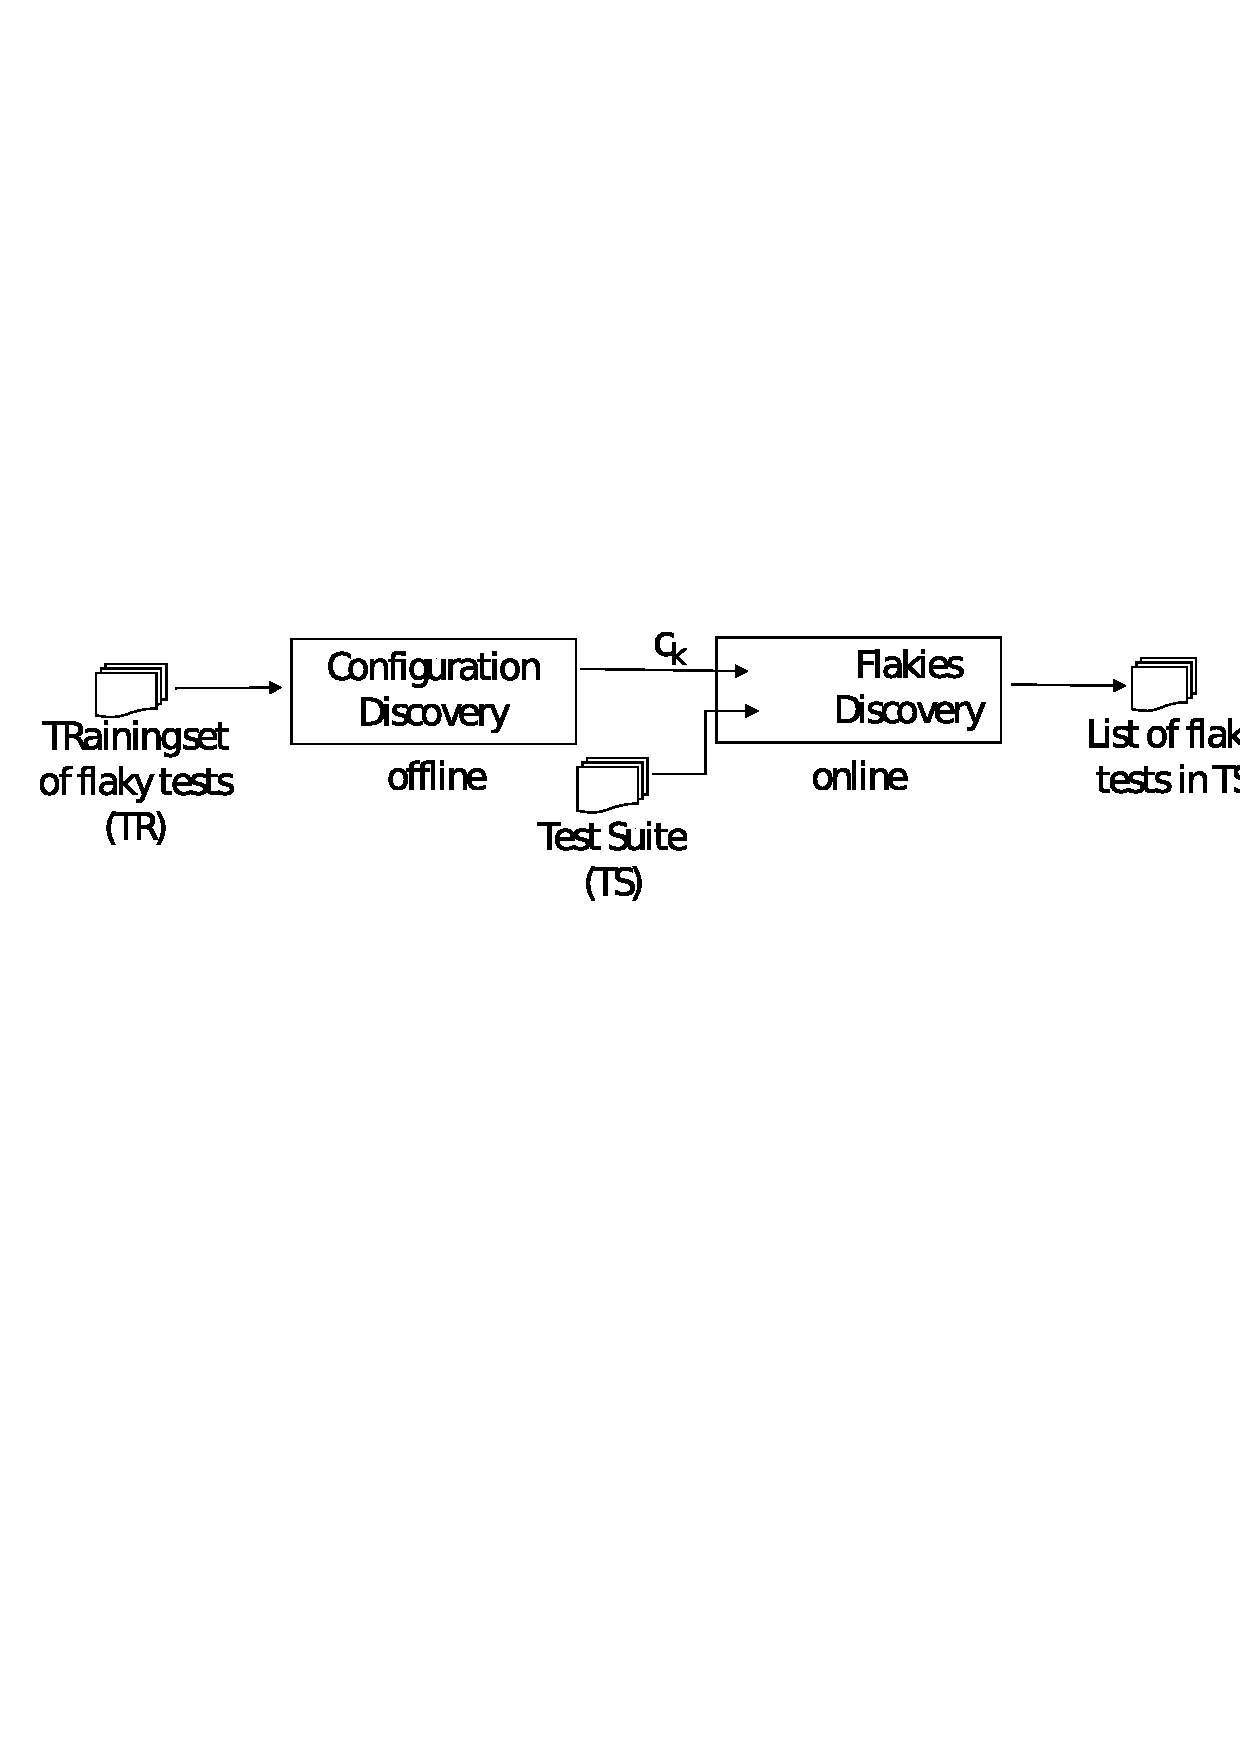
\includegraphics[trim=0 400 0 0,clip,width=0.75\textwidth]{figs/shaker.pdf}
    \caption{\tname's workflow.}
    \label{fig:workflow}
\end{figure}

Figure~\ref{fig:workflow} shows \tname{}'s workflow. \tname\ has an offline step and an online step. In the first \emph{offline} step, \tname{} uses a sample of tests known to be flaky to search for configurations of a noise generator. In the second \emph{online} step, \tname{} uses those configurations to find flaky tests in the test suite of a project provided as input. 

The following sections detail \tname. Section~\ref{sec:noise-generation} describes how an off-the-shelf tool can be used to generate noise in the execution environment. Section~\ref{technique:discovering-configurations} describes the offline step of generating configurations for a noise generator. Finally, Section~\ref{technique:finding-flakies} describes how \tname\ optimizes \rerun\ to find flaky tests efficiently.

%The input of \tname{} is a set of tests known to be flaky and the output is a set of configurations for creating noise in the execution environment. \tname{}'s workflow is comprised of two steps. 

%\Mar{@Leopoldo, vc. pode elaborar isto adicionando uma figura e detalhando as subsecoes?}
%\Leo{Ok, vou aproveitar nossa conversa para que eu entenda melhor cada etapa e assim possa explorar melhor o detalhamento do texto. E entao faco uma figura geral, sem problemas.}

\subsection{Noise Generation}
\label{sec:noise-generation}

A noise generator is a tool to create load. For example, a noise generator can spawn ``stressor'' tasks that can influence the execution environment where tests will be executed. Existing tools provide different choices of target for noise generation. We focused on CPU and memory options as we empirically found that they influence detection of test flakiness (see Section~\ref{sec:answer-rqone}). We used the \sng{}~\cite{stress-ng} tool to create CPU and memory load. 
We used the following options:

\begin{itemize}[topsep=.2ex,itemsep=.2ex,leftmargin=0.8em]
    \item \textbf{--cpu $n$}. Starts $n$ stressors to exercise the CPU by working sequentially through different CPU stress methods like Ackermann function or Fibonacci sequence.
    \item \textbf{--cpu-load $p$}. Sets the load percentage $p$ for the \textit{--cpu} command.
    \item \textbf{--vm $n$}. Starts $n$ stressors to allocate and deallocate continuously in memory.
    \item \textbf{--vm-bytes $p$}. Sets the percentage $p$ of the total memory available to use by the tasks created with option~\textit{--vm}.
\end{itemize}

For example, the command \CodeIn{stress-ng --cpu 2 --cpu-load 50\% --vm 1 --vm-bytes 30\%} configures \sng{} to run two CPU stressors with 50\% load each and one virtual memory stressor using 30\% of the available memory. The documentation of \sng{} can be found elsewhere.\footnote{\url{https://manpages.ubuntu.com/manpages/artful/man1/stress-ng.1.html}} 

In addition to the options listed above, \tname{} uses an option that we found important for finding flaky Android tests---the number of cores available for use by an Android emulator. This option can be used to restrict an Android emulator to run on a specified number of cores. 



%The rationale for selecting this option was that we evaluated \tname{} on Android and this option was found to be relevant for controlling the CPU load.

%\footnote{https://wiki.ubuntu.com/Kernel/Reference/stress-ng}, a specific tool designed to exercise various physical subsystems of a computer, your documentation has several examples and is simple to understand and \Fix{?}\Den{@Marcelo, a outra configuração que usamos não é bem uma ferramenta, apenas setamos a quantidade de cores que o emulador ira utilizar naquela execução, não sei explicar isso bem no texto}. 


\subsection{Step 1: Discovering Configurations}
\label{technique:discovering-configurations}

The goal of this step is to identify configurations of the noise generator that are more likely to reveal flakiness in a test suite. We search for configurations as a heavy-load could crash the emulator. It takes as input a set of tests \tr, \emph{known to be flaky}, and reports on output a list of configurations $c_k=[v_1,..., v_n]$. A noise generator is configured from a list of options $[o_1,...,o_n]$, with each option $o_i$ ranging over the interval $lo_i$-$hi_i$. Section~\ref{sec:noise-generation} describes which options are currently used. The flaky tests in \tr\ can be obtained with \rerun{}, \ie{}, by rerunning test sets of several applications for multiple times. Section~\ref{sec:objAndSetup} explains how we obtained the training set to evaluate \tname. To identify ``good'' configurations, it is necessary to define a metric for configuration quality. We use the symbol $\mathit{fit(c_k, \mathit{TR})}$ to denote the fitness value of configuration $c_k$ for the test set \tr. Fitness value is obtained by computing the average probability of detecting flakiness on \tr\ when the configuration $c_k$ is used for noise generation. 

\vspace{1ex}\noindent\textbf{Example.}~Consider that the set \tr\ contains three tests. A given configuration $c$ that detects flakiness in \tr\ with probabilities $\{0,2, 0.5, 0.0\}$ has $\mathit{fit}(c, \mathit{TR})$=$(0.2$+$0.5)/3$=$0.23$. These probabilities are obtained by running the test suite multiple times and computing the average number of failures. In this case, one test failed in 20\% of the reruns, another test failed in 50\% of the reruns, and another did not fail at all.

The search for noise configuration is realized in two stages. First, \tname{} samples configurations and generates a probability matrix characterizing the probability of each configuration to find flakiness in \tr. Second, \tname{} uses that matrix to search for sets of configurations. The following sections elaborate each of these steps in detail.

\subsubsection{Generation of probability matrix}
This step takes as input a set of flaky tests \tr\ and reports on output a probability matrix $M$, relating the tests in \tr\ and \emph{randomly-sampled} configurations in $K$ by their corresponding probabilities. The symbol $M[t][c]$ denotes the probability of configuration $c\in{}K$ detecting flakiness in $t\in{}\mathit{TR}$. To obtain approximate probability measurements, \tname{} runs each test several times on each sampled configuration. The probability measurement $M[t,c]$ is obtained by dividing the number of failures (of $t$ on $c$) found by the total number of reruns (of $t$ on $c$).

%\Mar{moved here...}
%\Fix{
%that maximize the probability of detecting flakiness. The rationale is that a %configuration can be, individually, very effective at detecting one subset of %flaky tests but not very effective at detecting flakiness for another subset %of flaky tests.  
%}

\subsubsection{\label{sec:search-configs}Search for sets of configurations} \tname{} offers two strategies to search for configurations. %: \greedy{}, and Minimum Hitting Set (\textbf{MHS}). 

The \textbf{\greedy{}} strategy sorts configurations according to their fitness value and  reports the top-$n$ configurations in the sorted list. The value $n$ is provided by the user. Note that this strategy does not offer guarantees that every flaky test will be detected. 

The Minimum Hitting Set (\textbf{MHS}) strategy takes that problem into account. MHS~\cite{10.1145/1150334.1150336} is a well-known intractable problem with efficient polynomial-time approximations~\cite{DBLP:journals/corr/Gainer-DewarV16}. To sum up, it enables \tname{} to obtain minimum sets of configurations (columns of the matrix) that detect the maximum number of flaky tests (rows in the matrix). Variations of the MHS problem exist considering weights and returning complete or partial (sub-optimal) solutions~\cite{seedselect}. \tname{} builds on the unweighted and complete MHS version, which takes a \emph{boolean} matrix as an input and produces a minimum hitting set encoding configurations as an output. We abstracted the probability matrix $M$ to only encode low or high likelihood of configurations detecting flaky tests. Intuitively, we are only interested in a configuration $c$ to detect flakiness of a certain test $t$ if the observed probability $M[t][c]$ is above a certain threshold. More precisely, \tname{} computes an abstract matrix $A$ defined as $A[t][c]$=$1$ if $M[t][c]>=\mathit{threshold}$, otherwise $0$. \tname{} runs MHS on the boolean matrix $A$. The goal is to find a set of configurations (columns in the matrix) that detects flakiness in tests (rows in the matrix). Note that, although MHS assures that all flaky tests are covered (\ie{}, a test would be detected with some configuration in the MHS), there is no guarantee that these tests are uniformly covered.

\vspace{1ex}\noindent\textbf{Example.} Figure~\ref{fig:msh-example} shows an illustrative example of the MHS procedure to discover configurations for detecting flakiness. The left-hand side of the figure shows the probability matrix $M$. The abstract matrix $A$ appears on the right-hand side. For space, we used a 3x4 matrix, \ie{}, the test suite contains three test cases and \tname{} sampled four configurations. In practice, these matrices are much bigger. The matrix on the left shows the probabilities of each configuration detecting flakiness on \tr. The matrix on the right-hand side is obtained using the abstraction function described above with a threshold value of 0.5. There are five hitting sets associated with the abstract matrix, namely $\{c_1, c_2, c_4\}$, $\{c_1, c_3, c_4\}$, $\{c_2, c_3, c_4\}$, $\{c_2, c_4\}$, $\{c_1, c_2, c_3, c_4\}$. The MHS algorithm is able to identify that the set $\{c_2, c_4\}$ is a minimal set that hits (\ie{}, covers) the tests in \tr. In this case, it is also the minimum.

 %when rerunning each test on each configuration for ten times, totalling 120 (=3x4x10) executions overall. 

\begin{figure}
    \centering
\begin{tabular}{ccccc}
    %\toprule
          &  $c_1$  & $c_2$   &  $c_3$  & $c_4$ \\
          \cline{2-5}
    $t_1$ &  0.1    &  0.6    &  0.5    &  0.2  \\
    $t_2$ &  0.6    &  0.6    &  0.1    &  0.2  \\
    $t_3$ &  0.1    &  0.1    &  0.1    &  0.5  \\
     \bottomrule
\end{tabular}
~
\hspace{1ex}
\begin{tabular}{ccccc}
    %\toprule
          &  $c_1$  & $c_2$   &  $c_3$  & $c_4$ \\
        \cline{2-5}
    $t_1$ &  0    &  1    &  1    &  0  \\
    $t_2$ &  1    &  1    &  0    &  0  \\
    $t_3$ &  0    &  0    &  0    &  1  \\
     \bottomrule
\end{tabular}
    \caption{Original probability matrix ($M$) and its abstracted version ($A$) using a threshold of 0.5. MHS($A$)=\{$c_2$, $c_4$\}.}
    \label{fig:msh-example}
\end{figure}


\subsection{Step 2: Discovering Flakies}
\label{technique:finding-flakies}

%To facilitate discussion, we use the term \rerunN{} to indicate a variation of \rerun{} that reruns tests in execution environments modified with a specified set of noise configurations.

Finally, \tname{} uses the configurations obtained on Step~1 to determine which of the tests the user provides are flaky. Figure~\ref{fig:workflow} illustrates the inputs and output of this step in the box named ``Flakies Discovery''. \tname\ reruns the test suite  on each configuration for a specified number of times and reports divergences on the test outputs. 

Note the tension between cost and effectiveness of \tname. The execution of a test suite under a loaded environment should be slower compared to a regular (noiseless) execution as different tasks are competing for the machine resources. Compared to \rerun{}, however, \tname{} may require less executions to detect flakiness. As result, the aggregate cost of detecting flakiness would be lower. 

%Section~\ref{sec:eval} evaluates this hypothesis.

%\multicolumn{1}{c}{

\begin{table*}[ht]
\caption{Apps and tests.}
\label{tab:Apps}
\small
\setlength{\tabcolsep}{6pt}
\begin{tabular}{rlrrrrlr}
\toprule
\# & App & \#Tests & \#Flakies & \CodeIn{@FlakyTest}(+/-) & \#Stars & GitHub URL (https://github.com/URL) & \multicolumn{1}{c}{SHA} \\ 
\midrule
1 & AntennaPod     & \numTestsAntenna{}   & 12 &  12/0    & 2.8k  & /AntennaPod/AntennaPod                & dd5234c \\
2 & \cellcolor{LightGray}AnyMemo        & 150   &  0   & 0/0      & 117   & /helloworld1/AnyMemo                  & 7e674fb \\
3 & Espresso & 14 & 1 & 1/0 & 1.1k & /TonnyL/Espresso & 043d028 \\
4 & FirefoxLite    & 70   & 15     &  15/3   & 220   & /mozilla-tw/FirefoxLite               & 048d605 \\
5 & Flexbox-layout &  232  & 1   & 0/231        & 15.5k & /google/flexbox-layout                & 611c755 \\
6 & Kiss           & 16    & 3   & 3/0      & 1.5k  & /Neamar/KISS                          & 00011ce \\
7 & \cellcolor{LightGray}Omni-Notes     & 10     & 0     &  0/0    & 2.1k  & /federicoiosue/Omni-Notes             & b7f9396 \\
8 & Orgzly         & 266   & 38      &  38/0  & 1.5k  & /orgzly/orgzly-android                & d74235e \\
9 & Paintroid      & 270   & 5        & 5/0 & 101    & /Catrobat/Paintroid                   & 1f302a2 \\
10 & \cellcolor{LightGray}Susi      & 17   & 0        & 0/0 & 2k    & /fossasia/susi\_android                   & 17a7031 \\
11 & \cellcolor{LightGray}WiFiAnalyzer   & 3     & 0  &  0/0       & 1k    & /VREMSoftwareDevelopment/WiFiAnalyzer & 80e0b5d \\ 
\midrule
Total   &  \multicolumn{1}{c}{-} & \totalTests\ & 75 (\percFlakyTestSds\%) & 74/234 &  \multicolumn{1}{c}{-} & \multicolumn{1}{c}{-} & \multicolumn{1}{c}{-} \\
\bottomrule
\end{tabular}
\end{table*}

\section{Objects of Analyses and Setup}
\label{sec:obj}
\label{sec:objAndSetup}

This section describes the methodology we used to build a data set of flaky tests (Section~\ref{sec:objects}) and the setup of \tname{} that we used to run the experiments (Section~\ref{sec:setup}).

\subsection{Objects}
\label{sec:objects}
We mined flaky tests from various GitHub projects to build a dataset to evaluate \tname{}. We used the following search criteria to select projects: 

\begin{enumerate}[leftmargin=1.2em]
    \item the project must be written in Java or Kotlin;
    \item the project must have at least 100 stars;
    \item the project must include tests in Espresso or UIAutomator;
    \item the project needs to be built without errors.
\end{enumerate}

We sampled a total of \numprojects\ projects that satisfied this criteria and used \rerun{} to find test flakiness. More precisely, we executed the test suite of these projects for \numReRuns{} times using a generic Android Emulator (AVD) with Android API version 28. As usual, we consider a test to be flaky if there was a disagreement in the outcomes (\ie, pass, fail, or error) across those runs. For example, we considered as flaky a test that passes in all but one run. To confirm that we could reproduce flakiness, we repeated the execution of each flaky test for 100 times. Section~\ref{sec:in-the-wild} shows results of running \tname{} to find other flaky tests on this same set of projects, \ie{}, flakies that went undetected with the aforementioned procedure and only \tname\ could detect.
Table~\ref{tab:Apps} shows the \numprojects\ projects we used. The column ``App'' shows the name of the Android app, the column ``\#Tests'' shows the number of Espresso or UIAutomator tests in that application, the column ``\#Flakies'' shows the number of flaky tests detected, column ``\CodeIn{@FlakyTest(+/-)} shows numbers x/y with x indicating the number of flaky tests we found that do \emph{not} contain the \CodeIn{@FlakyTest} annotation,\footnote{The \CodeIn{@FlakyTest} annotation is a JUnit test filter. It is used on test declarations to indicate JUnit to exclude those tests from execution (if a corresponding command is provided on input).} whereas y indicates the number of tests from the test suite containing the annotation \CodeIn{@FlakyTest} that we missed. Column "\#Stars" shows the number of stars that the project received on GitHub. Finally, columns ``GitHub...'' and ``SHA'' show the GitHub address and corresponding SHA prefix of the revision. 


\begin{figure}[t!]
    \centering
    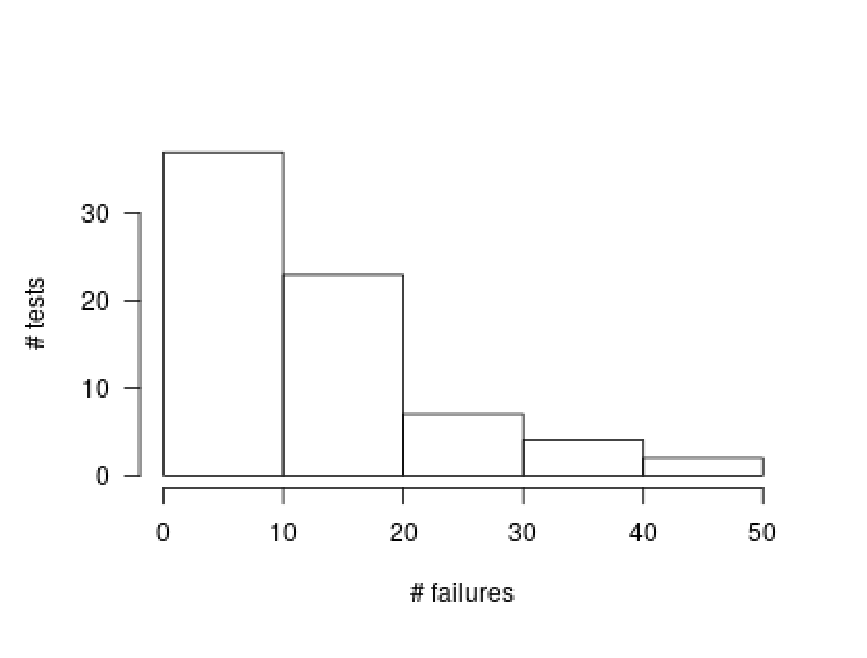
\includegraphics[trim=0 0 10 50,clip,width=0.35\textwidth,height=0.22\textwidth]{figs/histogram.eps}
    \vspace{-2ex}
    \caption{Histogram of test failures.}
    \label{fig:histogram-testfailures}
    \vspace{-3ex}
\end{figure}

We found flakiness in \numflakytestsds{} of the \totalTests\ tests we analyzed (=\percFlakyTestSds{}\% of the total). We found flaky tests in \numprojectsWithFlakies{} of the \numprojects{} apps. In two of these apps, namely \CodeIn{Espresso} and \CodeIn{Flexbox-layout}, we found only 1 flaky test. We highlighted the apps without flaky tests in gray color. Results also show that the \CodeIn{AntennaPod}, \CodeIn{FirefoxLite}, and \CodeIn{Orgzly} were the apps with the highest number of flaky tests, with 12, 15, and 38 flaky tests, respectively. These projects are among those with the highest number of test cases too, with 250, 70, and 266 tests, respectively. Curiously, we found that \CodeIn{Flexbox-layout} is one of the apps with the highest number of tests (232) and lowest number of flakies detected (1). Despite this evidence of determinism on the test suite, developers of this app chose to use the annotation \CodeIn{@FlakyTest} in \emph{all} tests. We inspected the code and it appears that developers used the annotation only for documentation---all tests in that app have that annotation and filtering test cases in that state would result in no test executed.
% \Mar{@Denini, is there some strong signal that explains why @FlakyTest was used. For example, use of network or sleeps?}. \Den{@Marcelo, eles fazem o testes 'mexendo' nos alementos diretamente na UIThread, acredito que seja isso. O paper do FlakShovel fala um pouco sobre isso: "The problem is that the operation of changing the element order is performed on the UIThread and position values of the elements are computed asynchronously and updated to View when the computation is completed." @Leopoldo viu uns testes lá, acho que ele pode complementar; }
\CodeIn{Flexbox-layout} consists in a library for implementing widgets that adhere to the CSS Flexible Box Layout module using the \CodeIn{RecyclerView} widget, which allows displaying lists and grids in Android applications. Tests rely heavily on checking list/grid elements, which are typically computed in worker threads, that require synchronization to be posted to the Main Thread. 

Figure~\ref{fig:histogram-testfailures} shows a histogram of number of failures for the \numflakytestsds{} flaky tests we discovered using \rerun. Nearly 52.1\% of the flaky tests revealed failure in 10 or less executions. This number is reflected in the leftmost bar from the histogram. Intuitively, to capture those cases, one would need to rerun the test suite for five times given that the failure probability for that group of tests is 20\% (=10/50). 

\subsection{Setup}
\label{sec:setup}

To evaluate \tname{}, we need to define (1) the training set of test cases \tr\ that will be used to discover configurations (step 1) and (2) the testing set of test cases $\mathit{TS}$ that will be used to discover the flaky tests (step 2). For that, we divided our dataset containing \numflakytestsds\ flaky tests as follows. We randomly sampled \numflakytraining\ tests and added them to the training set. The remaining \numflakytesting\ tests were added to the testing set.

The configuration discovery step of \tname\ also requires a sample of random configurations that will constitute the columns of the concrete and abstract matrices. For that, we sampled 50 configurations uniformly distributed across the domains of the five parameters we analyzed (see Section~\ref{sec:noise-generation}): four parameters from \sng{} and one parameter from the AVD. To obtain probabilities for the concrete matrix $M$, we ran each test on each of these configurations for \numReRunstrainingLONG{} times. The result of this execution is a probability matrix with failure probability values 0, 0.33, 0.66, 1.0. To construct the abstract matrix $A$, we used a probability threshold of \threshold{}, \ie{}, values equal or above that level are set to 1 (true) and values below that level are set to 0 (false).


%To answer this question we first conduct a training phase, where we choose suitable configurations. Afterwards, we have the testing phase, where we combine configurations. To this end, we split our flaky tests dataset into a training set, consisting of \numTrainingSet{} tests, while the remaining \numTestingSet{} tests are used in the testing phase. 


%Realizamos uma busca manual no Github por "Android" ou "app" com os seguintes criterios: 1) o projeto é feito em Java ou Kotlin. 2) possuem Testes de interface grafica (Espresso ou UIAutomator) e 3) conseguissem "dar build". 


\section{Evaluation}
\label{sec:eval}
The goal of this section is to evaluate the effectiveness of \tname. We pose the following research questions.

\newcommand{\rqone}{Do tests fail more often in noisy environments than in regular (non noisy) environments?}

\newcommand{\rqtwo}{How repeatable is the discovery of flaky tests with a given noise configuration?}

\newcommand{\rqthree}{How effective is the search for configurations of the noise 
generator (e.g., \greedy\ and MHS) that \tname\ uses?}

\newcommand{\rqfour}{How effective is \tname\ to find flaky tests?}

\newcommand{\rqfive}{How effective is \tname\ to find \emph{new} flaky tests?}

\vspace{0.5ex}
\noindent\textbf{RQ1.} \rqone
\vspace{0.5ex}

The purpose of this question is to evaluate if executing tests in noisy environments has the effect of making tests fail more often. This is an important question because \tname\ builds on that assumption to detect flaky tests, so if results are positive, than \tname\ is likely to be useful. 

\vspace{0.5ex}
\noindent\textbf{RQ2.} \rqtwo
\vspace{0.5ex}

This question analyzes the variance of results obtained with a given configuration of the noise generator. If results are very non-deterministic then selecting configurations, as described on Section~\ref{sec:search-configs}, is helpless as results would be unpredictable. 

\vspace{0.5ex}
\noindent\textbf{RQ3.} \rqthree
\vspace{0.5ex}

This question evaluates the effect of the (configuration) search strategies proposed by \tname\ in their ability to detect flaky tests. More precisely, this question compares \greedy\, MHS, and Random search in their effect to detect flakiness.


\vspace{0.5ex}
\noindent\textbf{RQ4.} \rqfour
\vspace{0.5ex}

This question evaluates how \tname{} compares with \rerun\ to find the flaky tests in our data set. To answer this question, we measured how long \tname{} and \rerun\ took to discover all flaky tests and how quickly each technique finds most tests. 

\vspace{0.5ex}
\noindent\textbf{RQ5.} \rqfive
\vspace{0.5ex}

For fairness with \rerun, the previous question restricted the evaluation of \tname\ to the set of flaky tests that \rerun\ itself was able to discover within \numReRuns\ re-executions (see Section~\ref{sec:objAndSetup}). This question evaluates the ability of \tname\ to discover flaky tests not detected by \rerun\ in the same set of projects.

\vspace{0.5ex}
The following sections elaborate the answers to each of these questions.

%We used the same data set to solve the optimization problem and to test it, with this experiment. As usual, we divided the sets of "training" and "testing" flaky tests from the data set to avoid bias. 
%The purpose of this question is to evaluate \tname{} on a data set different---and larger---than the one used to discover load configurations. It allows us to measure 1) how quickly \tname{} finds new flaky tests compared to \rerun\ and 2) if it is able to find more flaky tests compared to \rerun.

\subsection{Answering RQ1: \rqone}
\label{sec:answer-rqone}

%\Mar{@Denini, a ideia aqui eh vc. rodar varias configuracoes distintas aleatorias e medir o score. Vc. vai reportar dois conjuntos: C1 e C2. C1 é um conjunto com o score de N execucoes normais e C2 é um conjunto com o score de N execucoes com estas configuracoes distintas. @Leopoldo, vc. usaria este resultado para rodar um experimento estatistico. Faz sentido?} 

The purpose of this question is to evaluate the effect of introducing noise in the environment where tests are executed. This question is important as \tname\ assumes there is such effect. To answer the question, we ran statistical tests to evaluate if there are differences in the rate of failures observed in noisy executions versus standard executions. 

%So, for instance, for a configuration where 50 tests failed, the rate is given by $50/75=0.67$. \Fix{is associated with 30 executions of the \numflakytestsds{} flaky tests from regular executions of our data set. }

As we evaluated the \emph{effect} of noise on the same data set, we used a statistical test that takes two paired distributions on input--one distribution associated with regular executions and one distribution associated with noisy executions. Each number in the distribution corresponds to the rate of failures in one execution of the test suite, \ie{}, the fraction of the \numflakytestsds\ tests from our data set that fails. We ran each test suite on each treatment for 30 times. Consequently, each distribution contains 30 samples. 
First, we ran a Shapiro-Wilk test to check if the data is normally distributed. The p-values of this test are higher than the traditional threshold of $\alpha=0.05$. As such, we cannot reject the null hypothesis that the data is normally distributed with 95\% confidence. 
Given that both data sets are normally distributed, we used the paired t-test parametric statistical hypothesis test to check if there is difference in the measurements. 
The null hypothesis ($H_0$) is that the measurements are the same, that is, introducing noise does \emph{not} impact rate of failure. The test indicated that we could reject $H_0$ with 99\% confidence as the p-value is less than $0.01$. 
Since the distributions were different, we proceeded to evaluate the effect size. For that, we used Cohen's d to measure the difference in group means in terms of standard deviation units. 
This is given by $d=(\mu_1$-$\mu_2)/\sigma$, where $\mu_1$-$\mu_2$ is the difference over the two means from the sample data and $\sigma$ is the standard deviation of the data. 
The magnitude of the effect varies with the value of $d$, ranging from very small ($<$0.01) to huge ($>$2.0)~\cite{effect-sizes-cohen}. 
We obtained a value of $d=2.52$, which indicates that the effect of introducing noise was huge. 
%\Fix{We need to update this figure, and check whether the explanation needs to be adjusted}

Figure~\ref{fig:historgram-random} shows histograms for the distributions of values associated with noisy and noiseless runs. Note that, although some configurations manifest a relative small number of failures (0.15-0.2 range), most executions with noisy configurations raise more failures in tests. The average rate of failures in a noisy execution is 0.37. In contrast, regular executions have average failure rate of 0.09, which is substantially smaller compared with that of noisy runs.
\begin{figure}[t!]
    \centering
    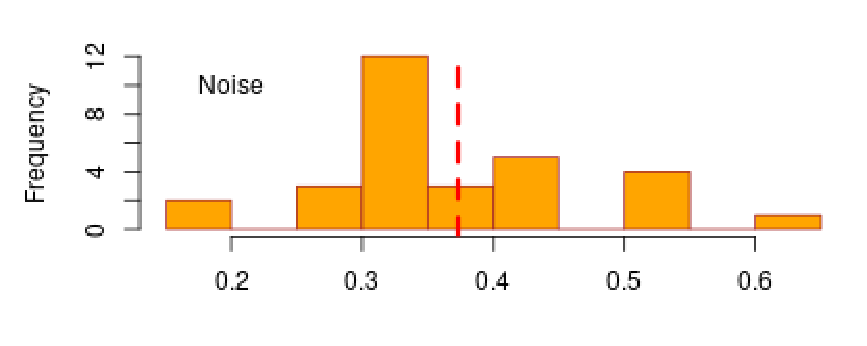
\includegraphics[width=0.4\textwidth]{figs/hist-failures-noise.eps}
    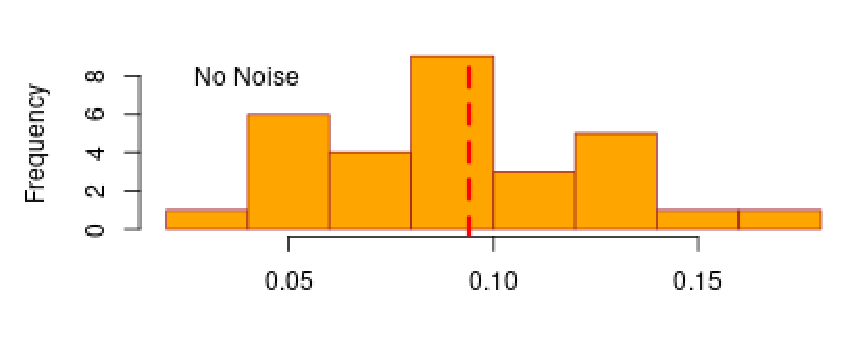
\includegraphics[width=0.4\textwidth]{figs/hist-failures-nonoise.eps}
    \vspace{-3ex}
    \caption{Histograms of ratio of failures for execution with and without noise. Vertical lines show average value.}
    \label{fig:historgram-random}
\end{figure}
To sum up: 
\begin{center}
\begin{tcolorbox}[enhanced,width=3.4in,center upper,drop shadow southwest,sharp corners]
\emph{Summary:}~Results indicate that introducing noise in the environment increases the ratio of failures in test suites with time-constrained test cases.
\end{tcolorbox}
\end{center}

\subsection{Answering RQ2: \rqtwo}
\label{sec:answer-rqtwo}

The goal of this question is to evaluate how repeatable are the results obtained with a given configuration. If results obtained with two runs of the test suite with the same configuration are very different, then choosing configurations randomly would be no worse than systematically searching for configurations as described on Section~\ref{technique:discovering-configurations}. 

To answer this question, we randomly selected 15 noise configurations and run the test suite on each one of them for 10 times, measuring the percentage of failures detected on each execution. For each one of the 15 configurations, we generated a distribution with 10 samples, where each sample indicates the percentages of failures detected on a given configuration. 

\begin{figure}[t!]
    \centering
    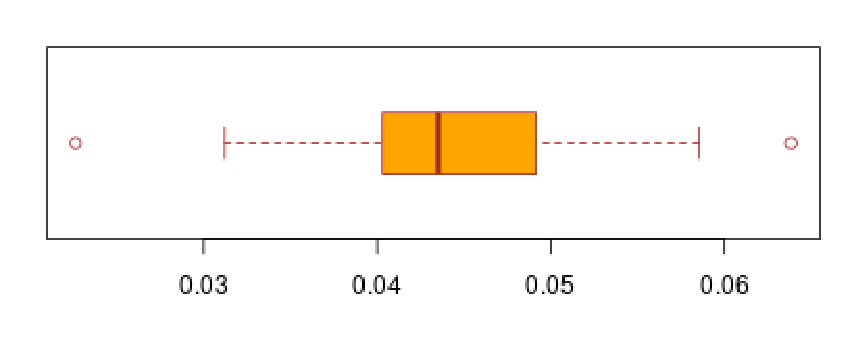
\includegraphics[width=0.4\textwidth]{figs/sd-random.eps}
    \vspace{-2ex}
    \caption{\label{fig:standard-deviations}Standard deviations of distributions of 10 reruns on each of the 15 randomly-selected configurations.}
    \vspace{-3ex}
\end{figure}

Figure~\ref{fig:standard-deviations} shows a boxplot associated with the standard deviations of these 15 distributions. Results indicate that the average and median standard deviation is $\sim$.04, indicating that the average difference in measurements is not superior to 8\% (avg\textpm$\sigma$ for a 95\% confidence interval) of the total number of flaky tests found. We conclude that:

\begin{center}
\begin{tcolorbox}[enhanced,width=3.4in,center upper,drop shadow southwest,sharp corners]
\emph{Summary:}~Despite the non-deterministic nature of the noise generation process, we observed relatively similar rates of failures across multiple executions of the same noise configuration. 
\end{tcolorbox}
\end{center}


\subsection{Answering RQ3: \rqthree}
%The probability matrix relates configurations with the flaky tests from the training set by the probability of a given configuration detecting flakiness on a given test. The focus of this research question is on step 2. 
%Section~\ref{sec:setup} shows how this set of random configurations is obtained.
%\footnote{The configurations are uniformly sampled from the configuration space. The configuration space consists of the Cartesian product of the domains of variables that control the generation of noise.}. 

Recall that \tname{} selects configurations in two steps (see Section~\ref{technique:discovering-configurations}). First, it generates a probability matrix and then it selects configurations from that matrix. This research question evaluates the effectiveness of the configuration selection strategies \tname{} uses. More precisely, it evaluates the ability of different techniques to select configurations. 

We evaluated three strategies for selecting configurations, namely, (i) MHS, (ii) Greedy, and (iii) Random. Recall that MHS is the technique that finds the smallest set of configurations whose execution of the test suite is capable of detecting all flaky tests from the training set (as per their associated probabilities in the abstract matrix). Greedy is the technique that selects configurations with maximum individual fitness scores (see Section~\ref{technique:discovering-configurations}). Random serves as our control in this experiment. It is the technique that randomly selects configurations regardless of their scores. Both Greedy and Random select the same number of configurations as MHS. 

%The combined score associated with the execution of the \numflakytesting\ test cases in the testing set on each of these four configurations. () 

The metric we used to compare techniques is the ratio of flaky tests detected when re-running the test suite against all configurations in the set associated with a technique. For example, let us consider that MHS produced four configurations. To obtain the score for that set, we execute the test suite four times, once for each configuration. Let us assume, we observe discrepancy in the outputs of 30 of the \numflakytesting{} flaky tests from the testing set. In that case, the score associated with the configuration set will be 0.75
~(=30/\numflakytesting{}). 


%For the \emph{training set} we used, MHS produced four configurations. After generating the configuration sets, we executed the test suite for \numExecutionsRQThree{} times on the \emph{testing set}, measuring the average fitness scores, \ie{} the percentage of flaky tests revealed. To illustrate, suppose MHS produces a set with four configurations. 

%\Den{@Marcelo, colocar um grafico de barras contendo todas as configurções e seus scores parece ser uma boa opção?}
%\Mar{Acho uma boa ideia, mas a gente precisa de mais execucoes para o histograma fazer sentido. Digamos 50 execucoes...}

We ran a statistical test to evaluate if there are differences in the
measurements obtained by MHS, Greedy, and Random. The metric used was the fitness score, as described above, \ie{}, we measured the ratio of flaky tests detected when using each selection strategy. We ran each technique for \numExecutionsRQThree{} times, so each distribution of measurements contain \numExecutionsRQThree{} samples.

As for RQ1, we ran a Shapiro-Wilk test to check if the data is normally distributed. We found that the p-values are above $\alpha=0.05$, therefore we concluded that the data is normally distributed. We then used Bartlett's test to check the homogeneity of variances, which reveals that the samples come from  populations with the same variance.
% \Mar{Unclear why Bartlett is necessary for (precludes) ANOVA.} 
% \Leo{I based myself on the documentation for the one-way ANOVA SciPy function, which states that we need to check for homoscedasticity, which is verified by Bartlett's test. See comment on LaTeX source.}
% The ANOVA test has important assumptions that must be satisfied in order for the associated p-value to be valid.
%     The samples are independent.
%     Each sample is from a normally distributed population.
%     The population standard deviations of the groups are all equal. This property is known as homoscedasticity.
As such, we chose to use the one-way ANOVA (ANalysis Of VAriance) parametric test to check statistical significance of the sample means by examining the variance of the samples. The null hypothesis ($H_0$) is that there is no variation in the means of sample measurements, which would indicate that there is no impact on changing selection strategies. 
The test reveals that there are statistically significant differences among treatments at the $p<0.01$ level (ANOVA F($2$,$27$)=$66.83$, $p<0.01$).
% \Mar{to clarify: confused about the role of ANOVA (as we do a post-hoc analysis later) and whether or not results are contradictory as there are no difference is variances (even for random?)}.
% \Leo{From what I understand, Bartlett's just checks that data varies in a homogeneous way among the samples, but does not compare the samples directly. ANOVA does this, but since we have three groups we nee to do paired compsrisons} 
%However, we cannot determine which treatments are significantly different from each other only from ANOVA. 

\begin{table}[ht]
\caption{Post-hoc analysis for RQ3 --- Multiple Comparison of Means using Tukey HSD} % title of Table
\centering % used for centering table

\adjustbox{width={0.5\textwidth},totalheight={\textheight},keepaspectratio}{
\begin{tabular}{|*{7}{c|}} % 7 centered columns
    \hline
    Group 1 & Group 2 & Mean Diff. & p adj. & Lower & Upper & Reject \\
    %heading
    \hline % inserts single horizontal line
    \hline % inserts single horizontal line
    Greedy & MHS & 0.008 & 0.8352 & -0.0279 & 0.0439 & \textbf{False} \\ \hline
    Greedy & Random & -0.141 & 0.001 & -0.1769 & -0.1051 & \textbf{True} \\ \hline
    MHS & Random & -0.149 & 0.001 & -0.1849 & -0.1131 & \textbf{True} \\ \hline
\end{tabular}
}
\label{tab:tukey} % is used to refer this table in the text
\end{table}

We performed a post-hoc paired comparison to evaluate which of the techniques differ. For that, we used the Tukey HSD test to execute multiple pairwise comparisons.
Table~\ref{tab:tukey} shows the difference in means, the adjusted p-values, and confidence levels for all possible pairs. Columns p-values and confidence levels show that between-group differences are significant only when comparing Random to MHS and Greedy. However, statistically, results do reject the hypothesis that Greedy and MHS are significantly different.

%                  sum_sq    df          F        PR(>F)
% C(treatments)  0.140487   2.0  66.827696  3.498036e-11
% Residual       0.028380  27.0        NaN           NaN

% Multiple Comparison of Means - Tukey HSD, FWER=0.05 
% ====================================================
% group1 group2 meandiff p-adj   lower   upper  reject
% ----------------------------------------------------
% Greedy    MHS    0.008 0.8352 -0.0279  0.0439  False
% Greedy Random   -0.141  0.001 -0.1769 -0.1051   True
%   MHS Random   -0.149  0.001 -0.1849 -0.1131   True
% ----------------------------------------------------


To sum up: 
\begin{center}
\begin{tcolorbox}[enhanced,width=3.4in,center upper,drop shadow southwest,sharp corners]
\emph{Summary:}~Results indicate that there is advantage in selecting noise configurations based on their fitness scores as opposed to randomly picking them. However, there is no statistical support to claim significant differences between MHS and Greedy.
\end{tcolorbox}
\end{center}

\subsection{Answering RQ4: \rqfour}
\label{sec:answer:rqfour}

The goal of this research question is to evaluate \tname{}'s performance. To that end, we analyzed two dimensions: (i)~efficiency, \ie{}, how fast it finds flaky tests, and (ii)~completeness, \ie{}, what is the fraction of the set of known flaky tests the technique detects. The set of flaky tests to be detected corresponds to the test set, as defined on Section~\ref{sec:setup}. 

\begin{figure}[t!]
    \centering
    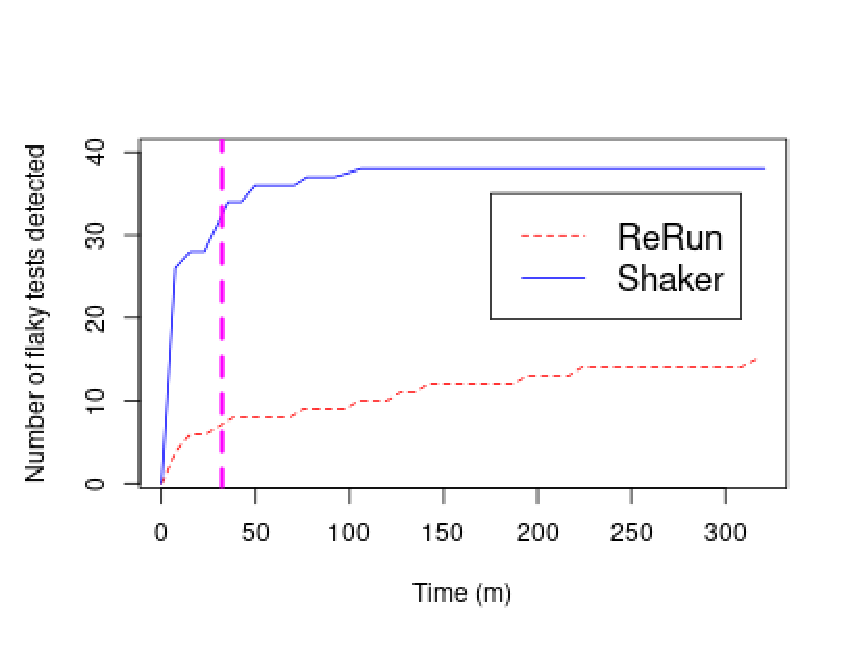
\includegraphics[width=0.4\textwidth]{figs/auc.eps}
    \vspace{-2ex}
    \caption{Progress over time of \tname\ and \rerun\ in detecting flaky tests.}
    \label{fig:auc}
    \vspace{-3ex}
\end{figure}

Figure~\ref{fig:auc} shows the progress of \tname\ and \rerun{} in detecting flaky tests over time. The x-axis denotes time in minutes whereas the y-axis denotes the number of flaky tests detected. The steep increase in the number of flaky tests detected by \tname\ indicates that it quickly discovers many flaky tests. For example, 26 of the \numflakytesting\ flaky tests failed (\ie{}, 65\% of the total) in the first execution of the test suite with \tname. Recall that the test set involves test cases of multiple projects. \rerun{} detected flakiness at a much slower pace, as reflected by the growth of its plot. \rerun\ needed 43 re-executions of the test suite and 316m (=5h16m) to reach saturation with \numFlakyDetectedReRun\ flaky tests detected (\ie{}, \percFlakyDetectedReRun{} of the total) whereas \tname\ needed 14 re-executions and 106m (=1h46m) to reach saturation with \numFlakyDetectedShaker{} flaky tests detected (\ie{}, \percFlakyDetectedShaker{} of the total). The vertical dotted line on Figure~\ref{fig:auc} marks the 32m point in time corresponding to 10\% of the time required by \rerun{} to saturate, which is the limit of the x-axis. In contrast, at that point, \tname{} had already found 34 of the flaky tests (\ie{}, 85\% of the total). 

We used the Area Under the Curve (AUC) as a proxy of effectiveness. Rothermel~\etal{}~\cite{Rothermel:ICSM99} pioneered the use of this metric to assess performance of test case prioritization techniques. The larger the area under the curve the better. For these progress plots, a higher area indicates higher ability to detect flaky tests and to detect them quickly. Intuitively, an optimal technique would detect all flaky tests in one execution and would have the AUC of a big trapezoid. Considering the plot from Figure~\ref{fig:auc}, the \rerun{} curve has an AUC of 3,491 where as the \tname{} curve has an AUC of 11,628, \ie{}, the area of \tname\ is 3.33x (=11,628/3,491) higher than that of \rerun. We used the \CodeIn{auc} function of the MESS library in R to compute the AUCs of these plots. That implementation uses the traditional trapezoidal integration method\footnote{https://www.lexjansen.com/nesug/nesug02/ps/ps017.pdf} to obtain AUCs. 

It is worth noting that, because of the increased load in the environment, one execution of the test suite with \tname{} is slower than one execution of the test suite with \rerun. The average cost of one execution of the test suite with \tname\ is 8m55s whereas the average cost of one execution of the test suite with \rerun\ is 7m38s.
Also note that \tname{} has the additional cost of finding configurations. However, this phase does not need to be executed as software evolves. Although the configurations that \tname{} finds can be calibrated with the inclusion of new projects and test suites for training, the proposal is to use the set of configurations found in test runs of any Android test suite. To sum up: 

%As \tname\ runs the test suite against four noise configurations, the average cost is 35m37s. 
\begin{center}
\begin{tcolorbox}[enhanced,width=3.4in,center upper,drop shadow southwest,sharp corners]
\emph{Summary:}~Results show that (1) \tname\ discovered many more flaky tests than \rerun{} (\percFlakyDetectedShaker{} versus \percFlakyDetectedReRun{}) and (2) it discovered these flaky tests much faster. \tname{} discovered 85\% of the total number of possible flakies in 10\% of the time \rerun\ took to find its maximum number of flakies.
\end{tcolorbox}
\end{center}


\subsection{Answering RQ5: \rqfive}
\label{sec:in-the-wild}

\begin{wraptable}[12]{r}{5cm}
\vspace{-4ex}
\caption{Number of new flaky tests found with \tname.}
\label{tab:new-tests}
\centering
\small
\begin{tabular}{lrr}
\hline
\toprule
\multirow{2}{*}{App} & \multicolumn{2}{c}{\# flaky tests} \\
\cline{2-3}
       & All & First 3 \\ 
\midrule
AntennaPod     & 27 & 20 \\ 
%AnyMemo        & 0       \\ 
%Espresso       & 0 \\ 
FirefoxLite    & 5 & 3\\ 
% Flexbox-layout & 2 \\ 
%Kiss           & 0  \\ 
Omni-Notes     & 4 & 3\\ 
Orgzly         & 14 & 10\\ 
Paintroid      & 10 & 8\\ 
%Susi           & 0       \\ 
WiFiAnalyzer   & 1 & 1\\ 
\midrule
Total:         & \numTotalNewFlaky{} & 45\\ 
\bottomrule
\end{tabular}
\end{wraptable}

% This experiment confirmed their robustness. \Den{@Marcelo, falta falar o caso para os apps Espresso e KISS, que nao encontramos nada novo, mas tem caso marcado como flaky no experimento anterior}\Leo{Nao entendi, nao seria o caso de mencionar junto com AnyMemo e Susi? Ou estes nao tinham nenhum flaky?}\Den{AnyMemo e Susi não tinham} 
 
We ran \tname\ on each project for 5h with the goal of finding additional flaky tests. Table \ref{tab:new-tests} shows the new flaky tests we found. We discarded tests with the \CodeIn{@FlakyTest} annotation from our search to avoid the risk of inflating our results given that developers already signaled a potential issue on those tests. As such, we needed to discard the project Flexbox-layout as all tests from that project contain that annotation.

Overall, we found new flaky tests in 6 of the 11 projects (10 if we exclude Flexbox-layout) and a total of \numTotalNewFlaky{} new flaky tests across these projects. \tname\ detected a total of 45 of these flaky tests in the first three runs of the test suite, confirming the behavior observed in the previous experiment when we showed that \tname\ could reveal most flaky tests very early during the search. We did not find any flaky tests on projects AnyMemo, Espresso, Kiss, and Susi. As per Table~\ref{tab:Apps}, note that the previous experiment we ran could not reveal any flaky tests on AnyMemo and Susi either. In contrast, we found one flaky test in Omni-Notes and WifiAnalyzer, projects that previously did not manifest test flakiness. It is important to recall that \percFlakyDetectedShaker\ of the \numflakytestsds\ flaky tests found by \rerun\ are also found by \tname\ (see Section~\ref{sec:answer:rqfour}). To sum up: 
\begin{center}
\begin{tcolorbox}[enhanced,width=3.4in,center upper,drop shadow southwest,sharp corners]
\emph{Summary:}~\tname\ revealed \numTotalNewFlaky\ new flaky tests that went undetected in \numRandomConfigs\ re-executions with \rerun.
\end{tcolorbox}
\end{center}

For each project where we found flaky tests, we opened issues on Github informing the detected flaky tests, explaining how we detected flakiness, and pointing to a shell script with instructions for reproducing our steps.\footnote{See \url{https://bit.ly/3dbqCZe} for a script for AntennaPod} 
% \footnote{See \url{https://gist.github.com/shaker-project/1639141948af4535b9180117824e4a61} for a script for AntennaPod} 
AntennaPod developers confirmed they are aware of flakiness for some of their tests, due to emulator performance when testing the Playback functionality. This is consistent with our discussion in Section~\ref{sec:example}. Some of those tests are ignored on their Continuous Integration systems. Nevertheless, we still detected flakiness in other tests, that developers considered as important to fix.\footnote{\url{https://github.com/AntennaPod/AntennaPod/issues/4194}}
Omni-Notes developers also modified their test suite to include the \CodeIn{@FlakyTest} annotation in the tests we reported as flaky.\footnote{\url{https://github.com/federicoiosue/Omni-Notes/issues/761}}


\subsection{Threats to validity}

Threats to the \emph{construct validity} are related to the appropriateness of the evaluation metrics we used. We used popular metrics previously used. For example, we used the ratio of detected flakiness, the number of flaky tests detected, and the Area Under the Curve (AUC) to evaluate the techniques.  

Threats to the \emph{internal validity} compromise our confidence in establishing a relationship between the independent and dependent variables. 
To mitigate this threat, we carefully inspected the results of our evaluation. In addition, we ran our experiments in different machines to confirm the impact of noise in detecting flakiness. 
%Finally, we contacted developers to confirm the flaky tests we detected. 

Threats to the \emph{external validity} relate to the ability to generalize our results. We cannot claim generalization of our results beyond the particular set of projects studied. In particular, our findings are intrinsically limited by projects studied, as well as their domains. 
%Although the studied projects are mostly written in Java\Leo{@Denini: Algum em Kotlin?}\Den{Sim, 3 apps}, we do not expect major differences in results if another language is used.\Leo{Se já tiver algum projeto em Kotlin, talvez não precise nem desta sentença.} 
The problems we found are related to task coordination. Nevertheless, future work will have to investigate to what extent our findings generalize to software written in other programming languages and frameworks (beyond Android and UI tests).


\section{Related Work}
\label{sec:related}
\label{sec:relatedwork}

%\Mar{discuss -->}\Fix{
%\cite{ifixflakies}
%\cite{idflakies}
%\cite{rootCausingflaky}
%%\cite{userInteractiveTests}
%\cite{refactoringOfTest}
%\cite{empiricallRevisiting}
%%}

We describe in the following recently related papers to ours.

\subsection{Empirical studies about bugs in test code}
Different empirical studies~\cite{Luo:2014:EAF:2635868.2635920,Vahabzadeh2015,Waterloo:2015,tran2019test} have attempted to characterize  the causes and symptoms of buggy tests, \ie{}, problematic tests that can fail raising a false alarm when there is no indication of a bug in the application code. This paper focuses on test flakiness, which is one of several possible types of test code issues.
For example, Vahabzadeh \etal{}~\cite{Vahabzadeh2015} mined the JIRA bug repository and the version control systems of Apache Software Foundation and found that 5,556 unique bug fixes exclusively affected test code. They manually examined a sample of 499 buggy tests and found that 21\% of these false alarms were related to flaky tests, which they further classified into Asynchronous Wait, Race Condition, and Concurrency Bugs. In principle all such problems can result in timing constraints that \tname{} could capture. Note, however, that we focused on Android, the diagnosis of defect is out of scope, and that \tname{} is a technique to find these issues whereas the aforementioned works manually analyze test artifacts.
%Recently, Tran et al.~\cite{tran2019test} studied test quality by surveying 19 practitioner's perceptions of test quality and conducting a mining study over the change history of 152 software projects, concluding that testers responsible for test execution are more concerned with comprehension of test cases rather than with their repeatability or performance.

Luo \etal{}~\cite{Luo:2014:EAF:2635868.2635920} analyzed the commit history of the Apache Software Foundation central repository looking specifically for flakiness. They analyzed 1,129 commits including the keyword ``flak'' or ``intermit'', and then manually inspected each commit. They proposed 10 categories of flakiness root causes and summarized the most common strategies to repair them. Many of the problems reported are related to timing constraints that could, in principle, be captured by \tname{}. We remain to investigate how \tname\ performs for software of different domains. Thorve \etal~\cite{thorve2018empirical} conducted a study in Android apps and observed that the causes of test flakiness in Android apps are similar to those identified by Luo~\etal{}~\cite{Luo:2014:EAF:2635868.2635920}. They also found two new causes as Program Logic and UI. 
%
Altogether, these studies show that test flakiness is prevalent and a potential deterrent to software productivity.

\subsection{Detection of test smells}

Code smells are syntactical symptoms of poor design that could result in a variety of problems. Test smells manifest in test code as opposed to application code. Van Deursen \etal{}~\cite{van2001refactoring} described 11 sources of test smells and suggested corresponding refactorings to circumvent them. More recent studies have been conducted on the same topic. Bavota~\etal{}~\cite{bavota2012empirical} and Tufano~\etal{}~\cite{tufano2016empirical} separately studied the sources of test smells as defined by Van Deursen~\etal{}~\cite{van2001refactoring}. They used simple syntactical patterns to detect these smells in code and then manually inspected them for validation. Bavota~\etal{} found that up to 82\% of the 637 test classes they analyzed contains at least one test smell. In related work, Tufano~\etal{} studied the life cycle of test smells and concluded that they are introduced since test creation---instead of during evolution---and they survive through thousands of commits. Waterloo~\etal{}~\cite{Waterloo:2015} developed a set of (anti-)patterns to pinpoint problematic test code. They performed a study using 12 open source projects to assess the validity of those patterns. 
Garousi~\etal{}~\cite{garousi2018we} prepared a comprehensive catalogue of test smells and a summary of guidelines and tools to deal with them. Test flakiness \emph{may} relate to test smells. For example, the use of sleeps are good predictors of flakiness~\cite{pinto-etal-msr2020,palomba2018automatic}; they induce time constraints that could be violated. We remain to investigate whether the extent to which static methods of flakiness prediction can improve the detection ability of \tname{}. For example, in principle, it is possible to instrument particular tests to initiate and terminate noise generation.

\subsection{Detection of flaky tests} 
%We are interested in identifying causes of flakiness as~\cite{Luo:2014:EAF:2635868.2635920,thorve2018empirical}, but we strive for automated and efficient detection of flakiness that could be applied, for example, to warn developers during evolution when they are about to add likely flaky tests. We remain to evaluate how our classifiers perform during evolution. We are particularly interested in understanding developers' reaction to the indication of potential flakiness produced by an IDE in contrast with the alternative approach that indicates flakiness in a report produced by Continuous Integration (CI) systems.

In principle, a test case should produce the same results regardless of the order it is executed in a test suite~\cite{DBLP:conf/issta/ZhangJWMLEN14}. Unfortunately, this is not always the case as the application code that is reached by the test cases can inadvertently modify static area and resetting the static area after the execution of a given test is impractical. Test dependency is one particular source of flakiness~\cite{Luo:2014:EAF:2635868.2635920}. Gambi~\etal{}~\cite{gambi2018practical} proposed a practical approach, based on flow analysis and iterative testing, to detect flakiness due to broken test dependencies. \tname{} is complementary to techniques for capturing broken test dependencies. It remains to investigate how a technique that forcefully modifies the test orderings (e.g.{}, discarding tests from test runs and modifying orderings of test execution) compares with the approach proposed by Gambi~\etal.

Bell~\etal{} proposed DeFlaker~\cite{bell2018d}, a dynamic technique that uses test coverage to detect flakiness during software evolution. DeFlaker observes the latest code changes and marks any new failing test that did \emph{not} execute changed code as flaky tests. The expectation is that a test that passed in the previous execution and did not execute changed code should still pass. When that does not happen, DeFlaker assumes that the changes in the coverage profile must have been caused by non-determinism. Note that DeFlaker is unable to determine flakiness if the coverage profile was impacted by change and the ability of DeFlaker to detect flakiness is bound by the ability of \rerun{} itself. Shi~\etal{}~\cite{ifixflakies} proposed iFixFlakies to find and fix flaky tests caused by broken test dependencies. \tname\ focuses on a different source of flakiness, which often relates to time-constraints, such as those brought by concurrency. Recently, Dong~\etal{}~\cite{dong2020concurrencyrelated} proposed FlakeShovel, a tool to detect flakiness in Android apps by monitoring and manipulating thread executions to change event orderings. It directly interacts with the Android runtime, instead of generating stress loads, as we did. We remain to evaluate how \tname\ compares with FlakeShovel. %Even though we only exercised \tname\ in the Android context, we believe that the approach can be applied in other domains.

%Machine learning has also been used to 

Purely static approaches have also been proposed to identify flaky tests~\cite{Herzig:2015,king2018,bertolino2020flaky,pinto-etal-msr2020}. An important benefit of these approaches is scalability. For example, it is possible to build services to proactively search for suspicious tests in open source repositories. On the downside, they only offer estimates of flakiness; re-execution is still necessary to confirm the issue. Herzig and Nagappan~\cite{Herzig:2015} developed a machine learning approach that mines association rules among individual test steps in tens of millions of false test alarms. Lam~\etal{}\cite{king2018} used Bayesian networks for flakiness classification. Pinto~\etal{}~\cite{pinto-etal-msr2020} used binary text classification (e.g.{}, Random Forests) to predict test flakiness. They used typical NLP techniques to classify flaky test cases---they tokenized the body of test cases, discarded stop words, put words in camel case, and built language models from the words associated with flaky and non-flaky tests. \tname{} is complementary to static techniques. We remain to evaluate how static classification techniques could be used to selectively run tests in a noisy environment.

%In contrast, our work aims at developing a lightweight flakiness predictor that learns from test code of flaky and non-flaky tests. We are aware of one only recent approach that takes a similar standpoint as we do (i.e.,~\cite{}). However, here, we derive a more comprehensive set of predictors and build a vocabulary of tokens, which is out of their scope.

%The works in~\cite{Herzig:2015,king2018} aim instead to build a \textit{static} predictor, as we also do here. The work in
%\Fix{-------------------------------------------- estou aqui}
%Bell~\etal{}~\cite{bell2018d} and Lam~\etal{}~\cite{lam2019idflakies} proposed different techniques to dynamically detect test flakiness. They require that test cases are executed (one or more times), aiming at optimizing the traditional approach used by practitioners of rerunning failed tests for a fixed number of times. For example, 


\section{Conclusions}
\label{sec:conclusion}
%Regression testing is an important quality assurance practice in software industry. 

Flaky tests are a huge problem in industry. Their presence makes it difficult for developers to unambiguously interpret the results of a regression testing cycle. This paper proposes \tname, a lightweight approach to detect flakiness in time-constrained tests by adding noise in the execution environment. For example, \tname\ adds stressor tasks to create load in the CPU and memory. We evaluated \tname\ on a sample of \numprojects\ Android apps. Results are very encouraging. \tname\ discovered many more flaky tests than \rerun{} (\percFlakyDetectedShaker{} and \percFlakyDetectedReRun{} of the total, respectively) and discovered these flaky tests much faster. In addition, \tname\ was able to reveal \numTotalNewFlaky\ new flaky tests that went undetected in \numRandomConfigs\ re-executions with \rerun. Our data sets and results are publicly available at \artifactUrl.

{\small
\noindent\textbf{Acknowledgements.}~This research was partially funded by INES 2.0, FACEPE grants PRONEX APQ 0388-1.03/14 and APQ-0399-1.03/17, CAPES grant 88887.136410/2017-00, FACEPE grant APQ-0570-1.03/14 and CNPq (grants 465614/2014-0, 309032/2019-9, 406308/2016-0, 409335/2016-9).
}

%\newpage
\IEEEtriggeratref{21}
\bibliographystyle{IEEEtran}
\bibliography{IEEEabrv,references}
    
\end{document}